\chapter{User Documentation}
\label{chap:user-documentation}

\section{Home}
\label{sec:user-documentation-home}
The home page is the initial page the users see after visiting the website (see Figure \ref{fig:user-documentation-home}). Users can navigate to the graphs page, which presents a comprehensive network of articles spanning the last three months. Additionally, they have access to the companies page, which provides a detailed listing of companies.

\begin{figure}[ht]
  \centering
  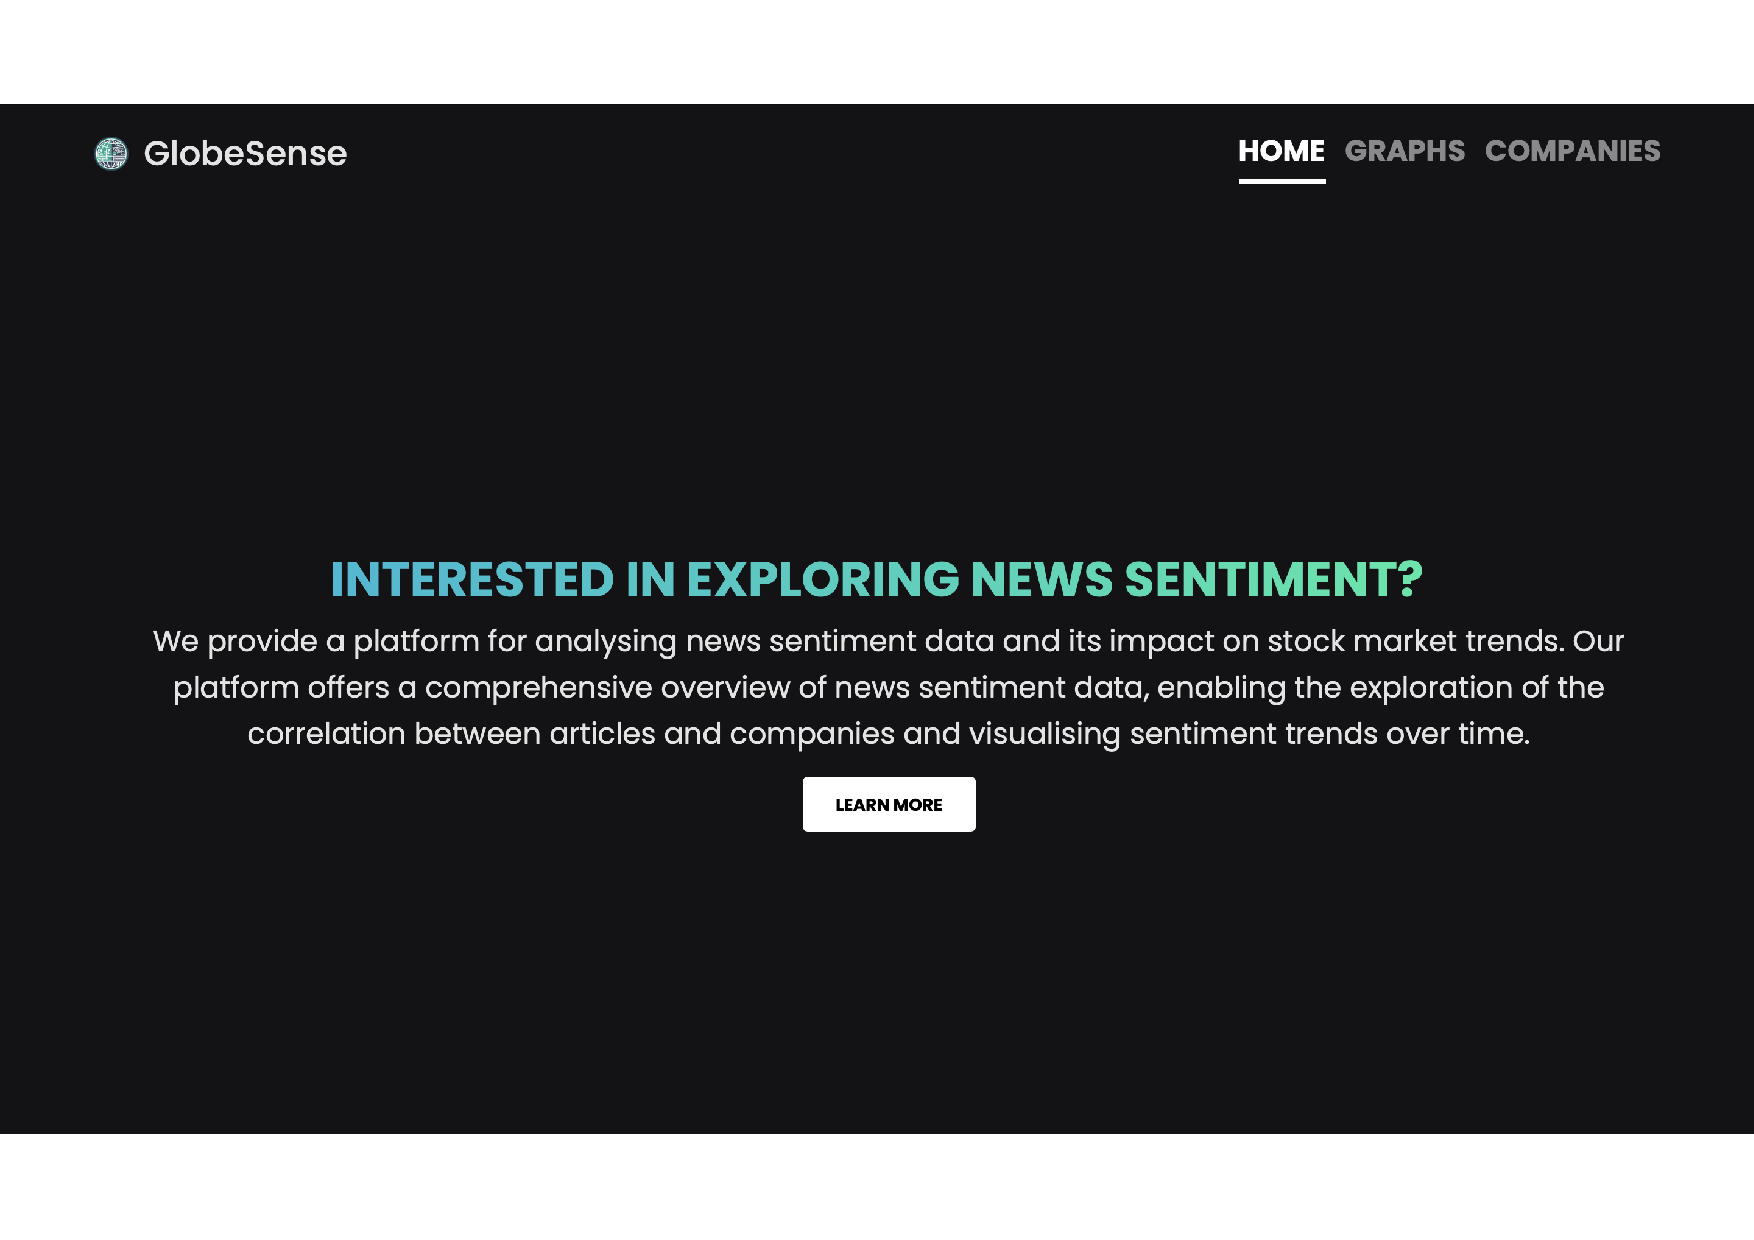
\includegraphics[width=\textwidth]{img/user/home-a.pdf}
  \caption{The website's home page briefly describing the project and its purpose.}
  \label{fig:user-documentation-home}
\end{figure}

\section{Graphs}
\label{sec:user-documentation-graphs}
The graphs page displays a network of all articles from the past three months. Each edge represents the sentiment of the company mentioned in the article, indicated by its colour. The article node's colour represents the average sentiment of all connected companies. Hovering over a node reveals its name if it is a company or its title if it is an article (see Figure \ref{fig:user-documentation-graphs}). Furthermore, neighbouring nodes are highlighted.

\begin{figure}[ht]
    \centering
    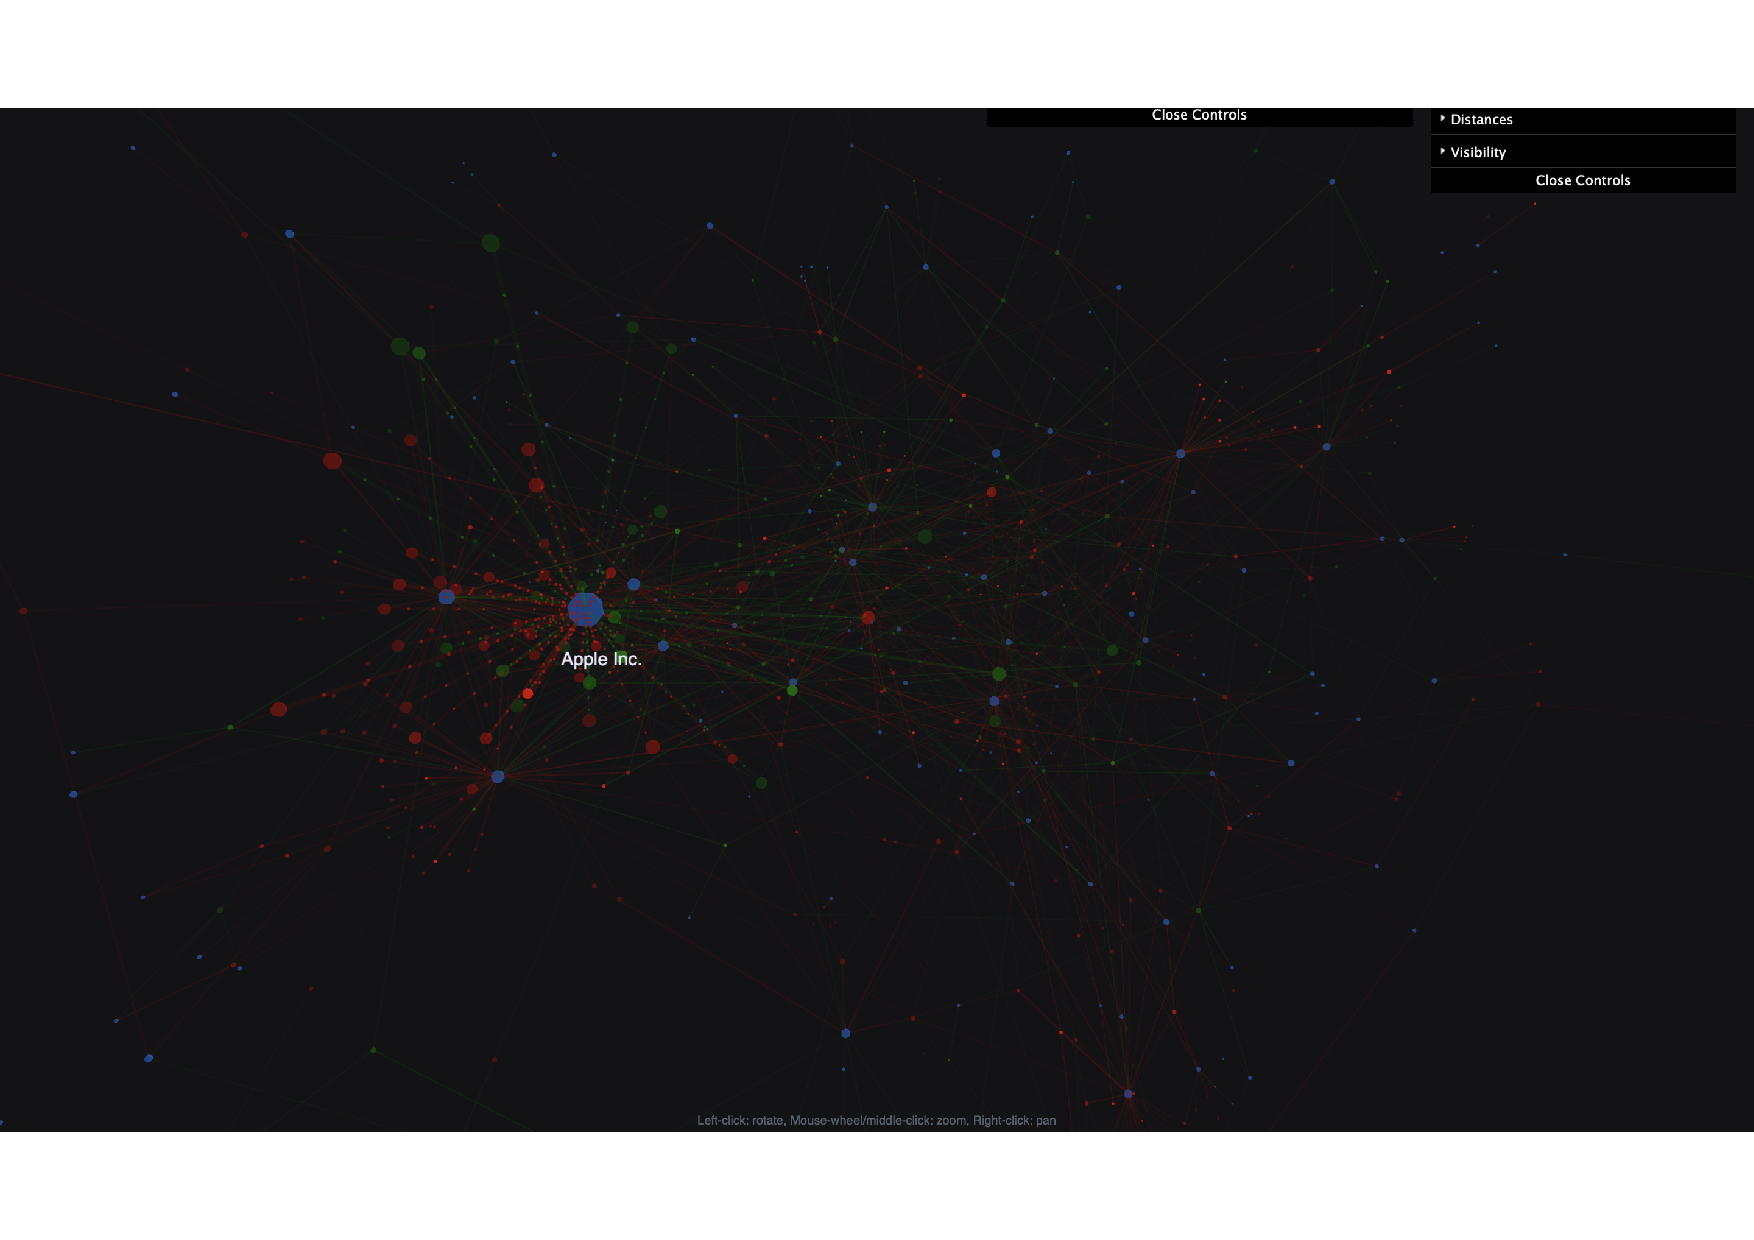
\includegraphics[width=\textwidth]{img/user/graphs-a.pdf}
    \caption{Users can see the network of all articles for the past three months by navigating to the graphs page.}
    \label{fig:user-documentation-graphs}
\end{figure}

\subsection{Control Panels}
\label{subsec:control-panel}
The control panels on the upper right side of the page are categorized into two types. The first type is the general control panel, specifically designed for managing the network graphs and encompasses the following features:
\begin{itemize}
    \item \textbf{Distances}
    \begin{itemize}
        \item \textbf{Positive distance} - regulates the distance of the edge with positive sentiment.
        \item \textbf{Neutral distance} - regulates the distance of the edge with neutral sentiment.
        \item \textbf{Negative distance} - regulates the distance of the edge with negative sentiment (see Figure \ref{fig:user-documentation-graphs-distances}). 
    \end{itemize}
    \item \textbf{Visibility}\footnote{Visibility filtering is not available when only neighbouring nodes are visible. Refer to its corresponding company graph page for specific node examination and filtering.}
    \begin{itemize}
        \item \textbf{Show only negative sentiment} - shows only the article nodes with negative sentiment (see Figure \ref{fig:user-documentation-graphs-only-negative}).
        \item \textbf{Show only neutral sentiment} - shows only the article nodes with neutral sentiment.
        \item \textbf{Show only positive sentiment} - shows only the article nodes with positive sentiment.
    \end{itemize}
\end{itemize}

Another control panel is available for node details, which appears upon left-clicking on an article node. It provides the following options:

\begin{itemize}
    \item \textbf{Article node}
    \begin{itemize}
        \item \textbf{Title} - the title of the article.
        \item \textbf{Published date} - the date when the article was published.
        \item \textbf{Author} - the author of the article.
        \item \textbf{Open article} - the link to the article.
        \item \textbf{Average sentiment} - the average sentiment of the article is based on the average sentiment of the companies mentioned.
        \item \textbf{Companies} - the list of companies mentioned in the article with their sentiment. It expands on details about the company and its sentiment in the article (see Figure \ref{fig:user-documentation-graphs-article}).
    \end{itemize}
    \item \textbf{Company node}
    \begin{itemize}
        \item \textbf{Company information} - the details about the company, such as ticker and link to the company's dashboard or graph page.
        \item \textbf{Articles} - the list of articles in which the company is mentioned with the sentiment of the company in the article (see Figure \ref{fig:user-documentation-graphs-apple-negative}).
    \end{itemize}
\end{itemize}

\subsection{Actions}
\label{subsec:actions}
\begin{itemize}
    \item \textbf{Left click} on a node involves zoom-in, then it will show only the neighbours of the clicked node.
    \item \textbf{Right click} on a node will show all nodes back.
    \item \textbf{Hover node} shows a name of the company or the title of the article and highlights the neighbours.
\end{itemize}

\begin{figure}[htbp]
    \centering
    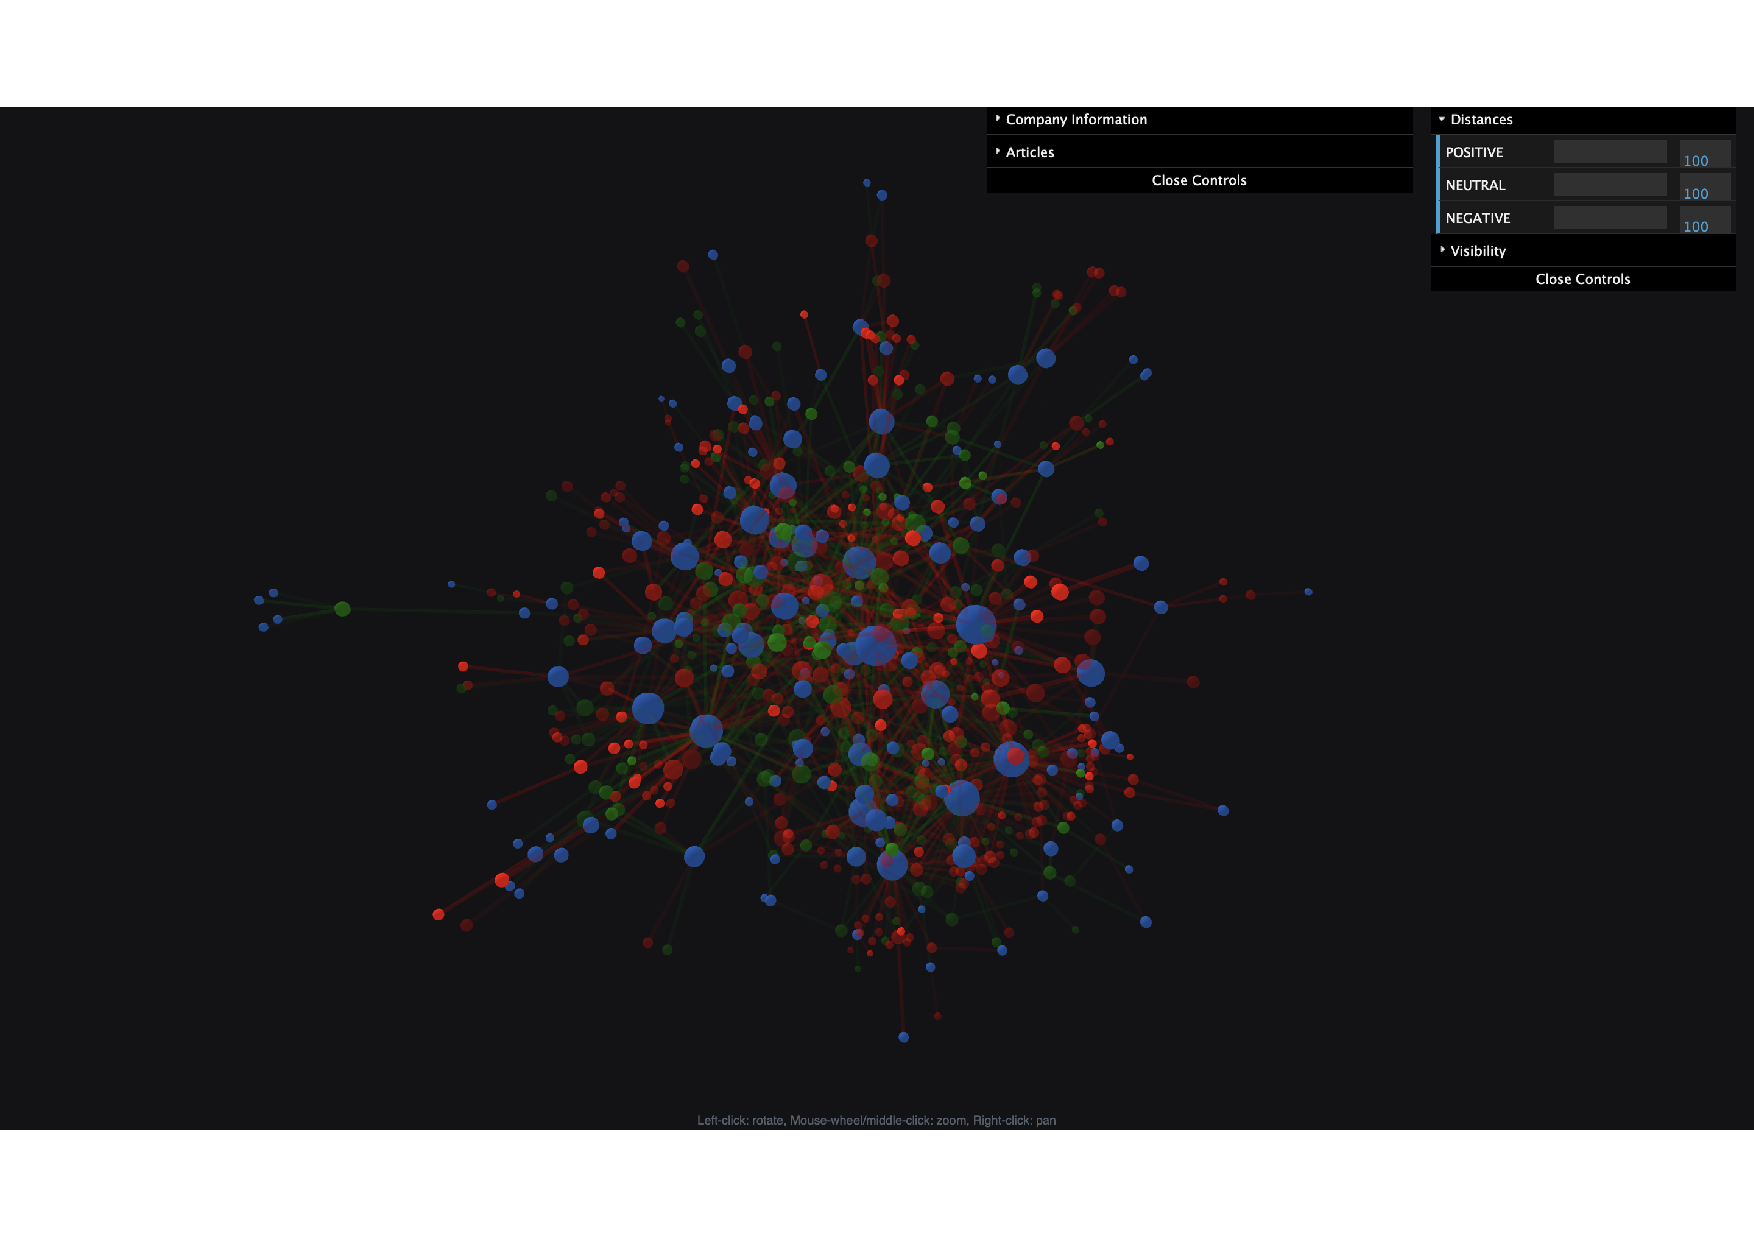
\includegraphics[width=\textwidth]{img/user/graphs-distances-a.pdf}
    \caption{The control panel managing edge distances. This involves selecting edges with sentiments and regulating them with values ranging from 100 to 3000. The image shows the network with the edge distances set to 100.}
    \label{fig:user-documentation-graphs-distances}
\end{figure}

\begin{figure}[htbp]
    \centering
    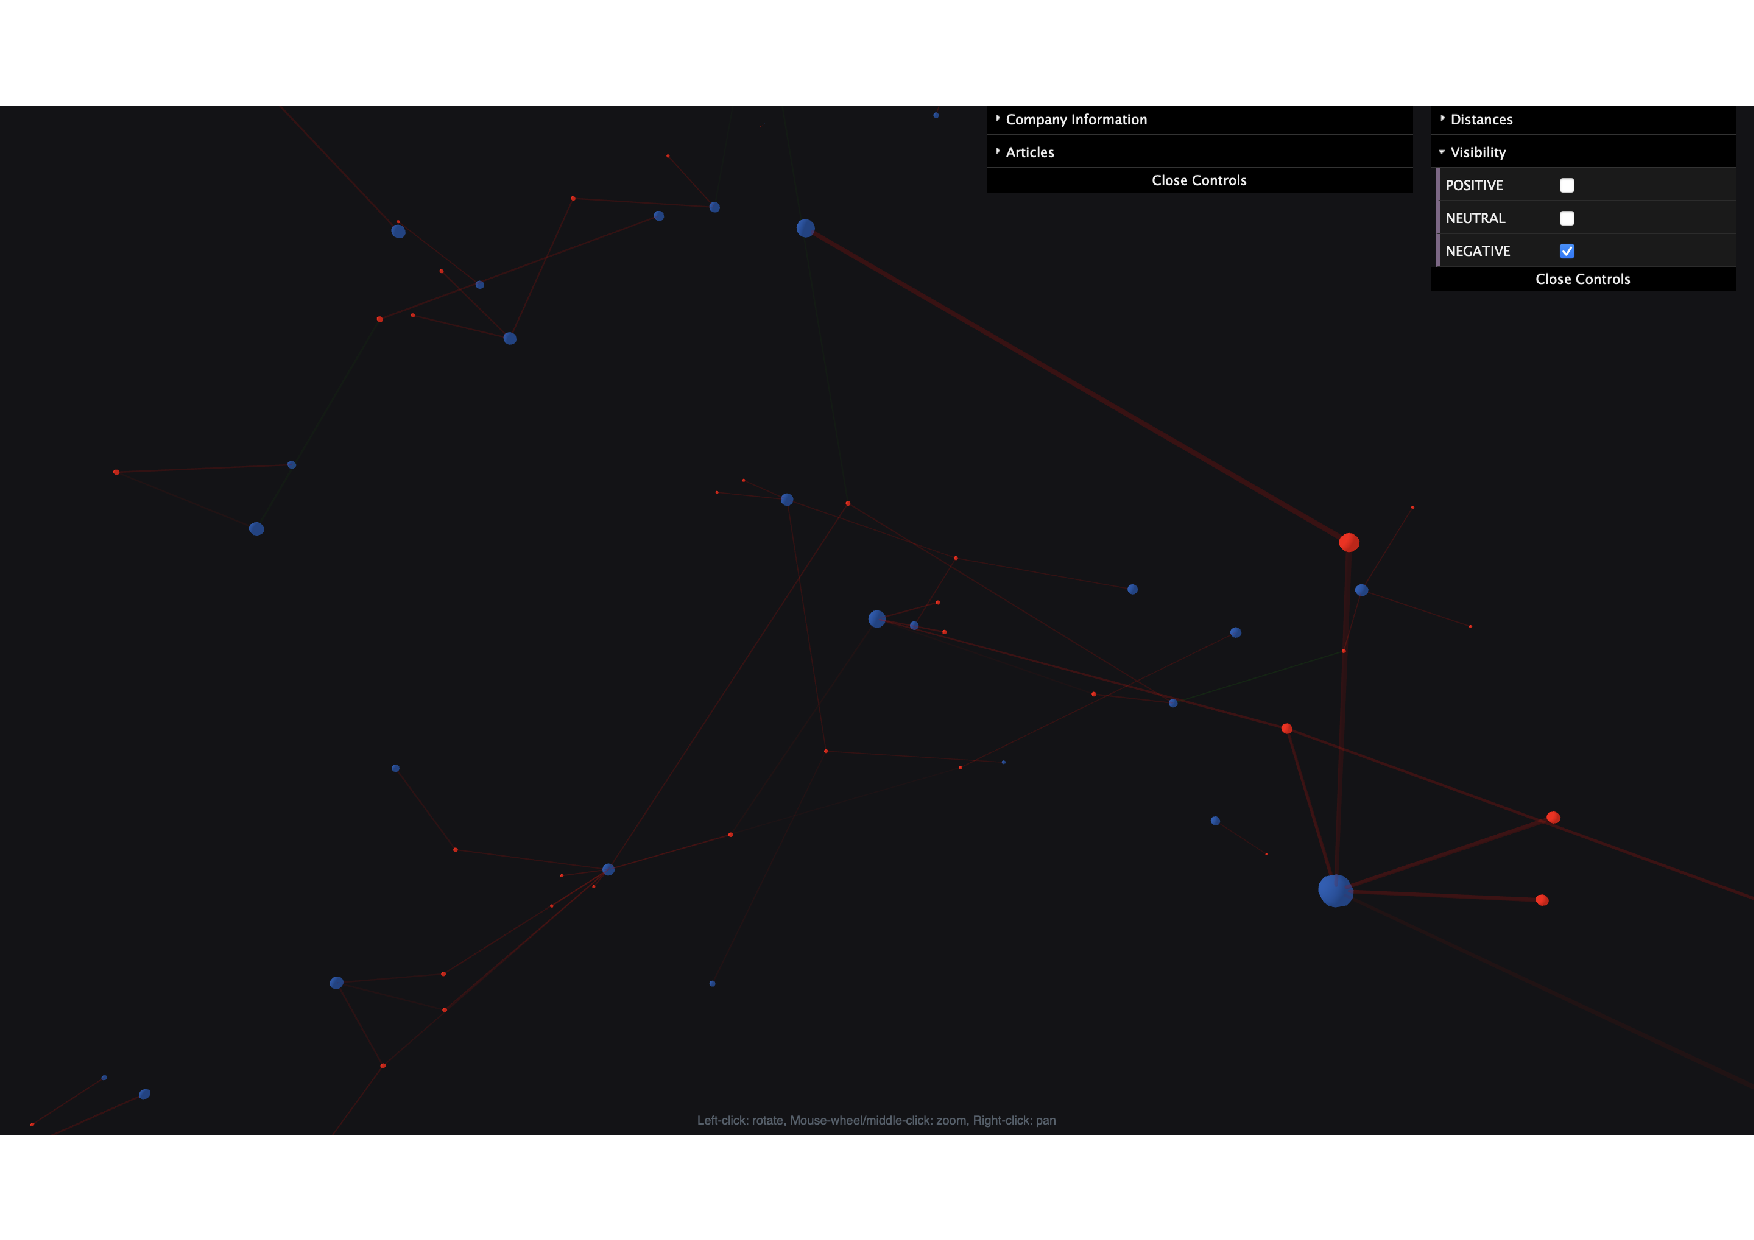
\includegraphics[width=\textwidth]{img/user/graphs-only-negative-a.pdf}
    \caption{After right-clicking, all nodes will be displayed back. The neutral and positive sentiments of the article nodes were turned off through the control panel. If there is an edge to the article node, then it remains to be visible.}
    \label{fig:user-documentation-graphs-only-negative}
\end{figure}

\begin{figure}[htbp]
    \centering
    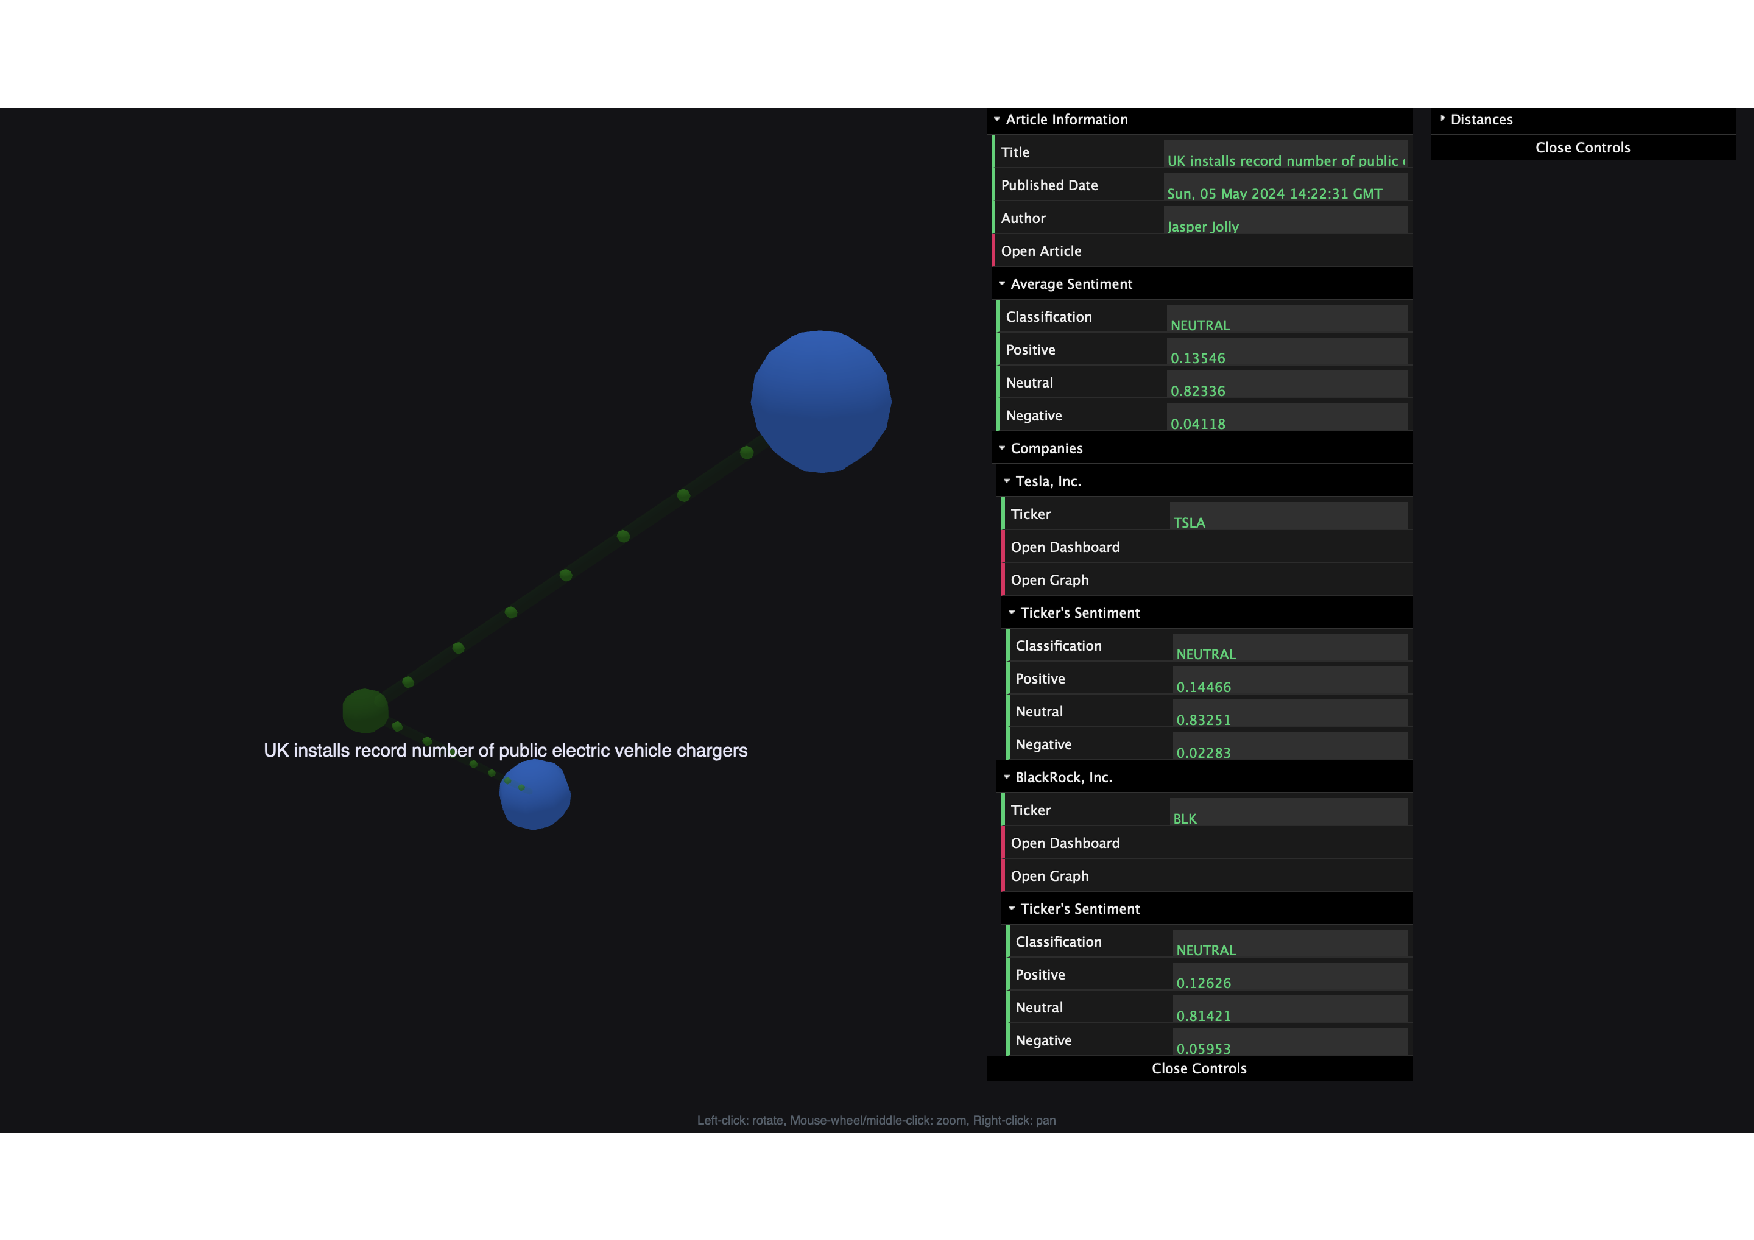
\includegraphics[width=\textwidth]{img/user/graphs-article-a.pdf}
    \caption{After left-clicking on an article node, the control panel could be expanded with further information, such as listing all companies mentioned in the article with their sentiment as well as the average sentiment of the article and more detailed information about the title, date, author, and link to the article.}
    \label{fig:user-documentation-graphs-article}
\end{figure}

\begin{figure}[htbp]
    \centering
    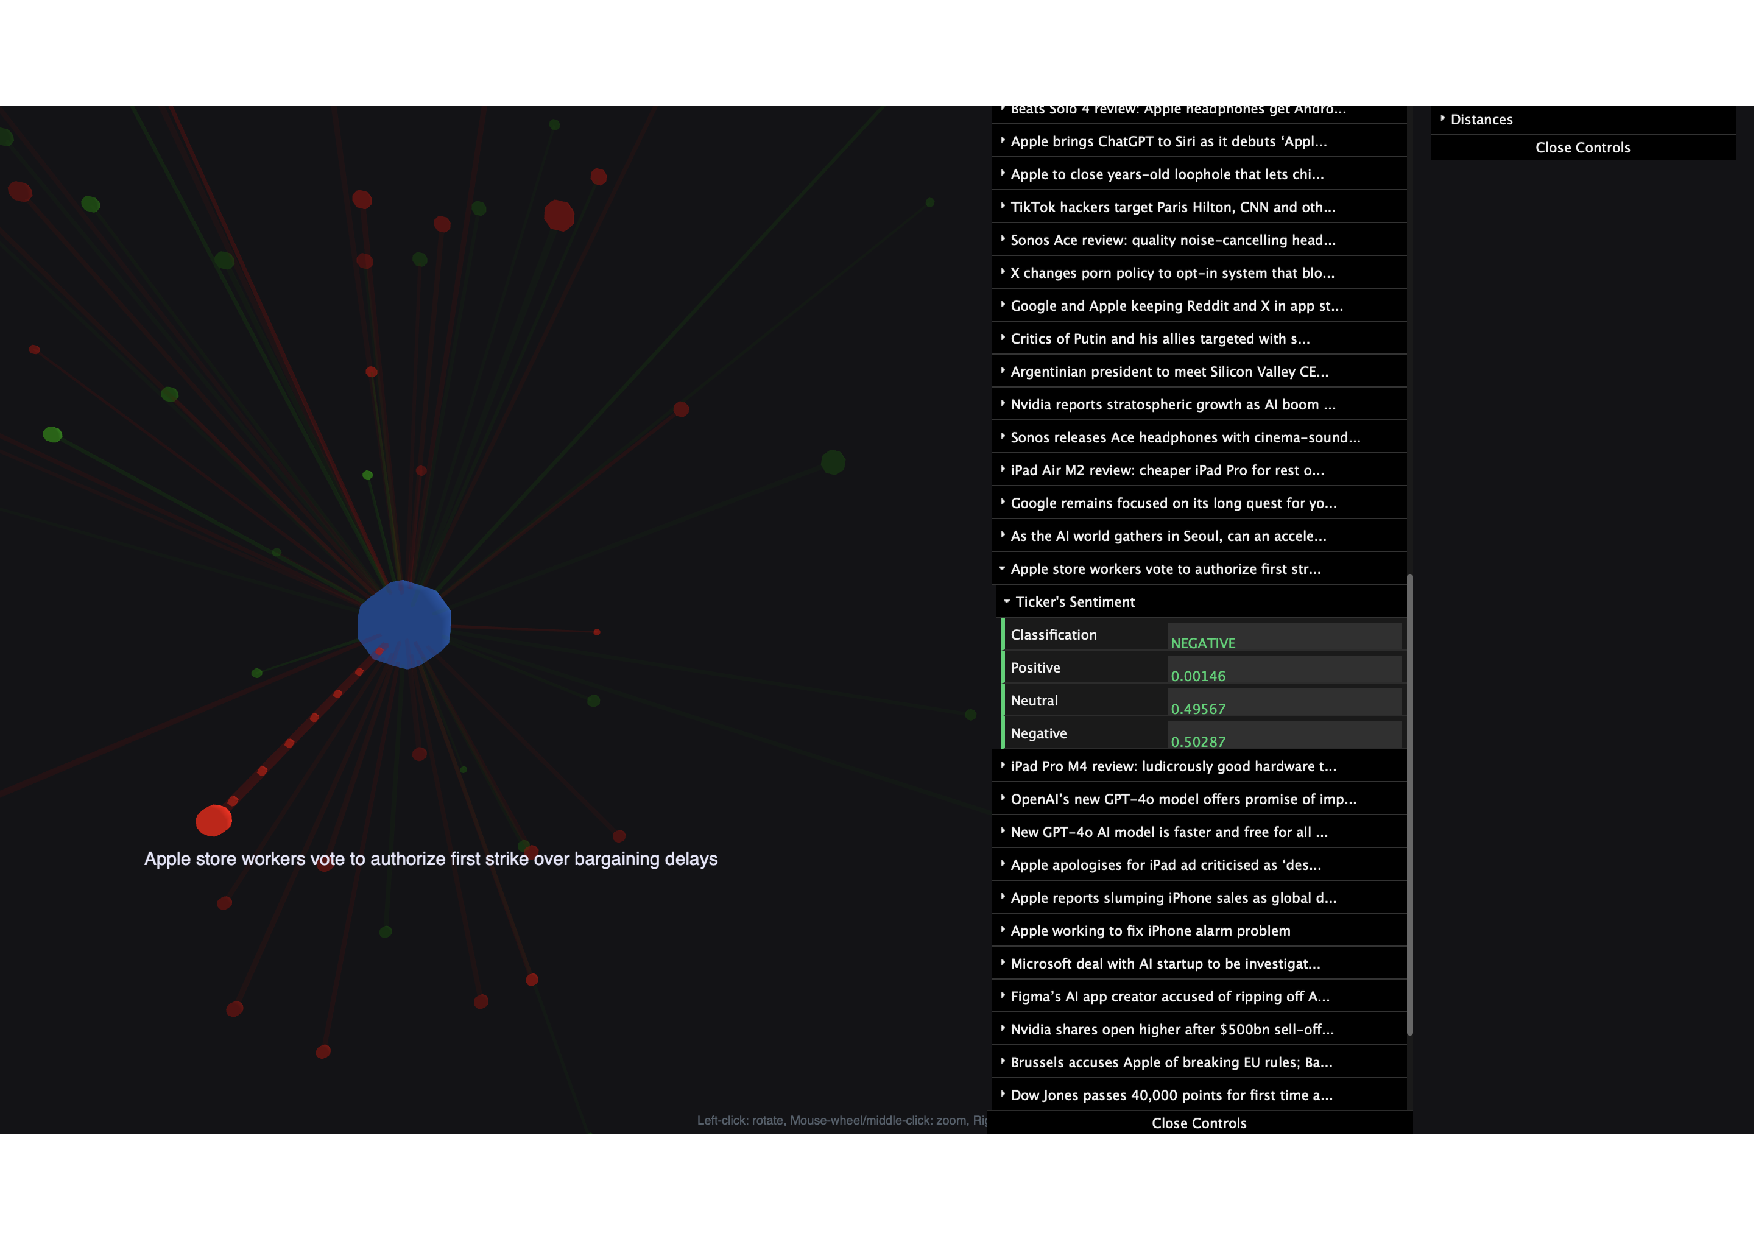
\includegraphics[width=\textwidth]{img/user/graphs-apple-negative-a.pdf}
    \caption{Apple Inc. node with its neighbours after left click. The list of articles in which it is mentioned additionally provides the values of its sentiment, which is Apple's sentiment in that article. The article's colour indicates a negative average sentiment.}
    \label{fig:user-documentation-graphs-apple-negative}
\end{figure}

\newpage

\section{Companies}
\label{sec:user-documentation-companies}
The companies page allows the users to search for a company by its name or stock symbol. The users can also navigate to the company's dashboard or graph page (see Figure \ref{fig:user-documentation-companies-search}).

\begin{figure}[htbp]
    \centering
    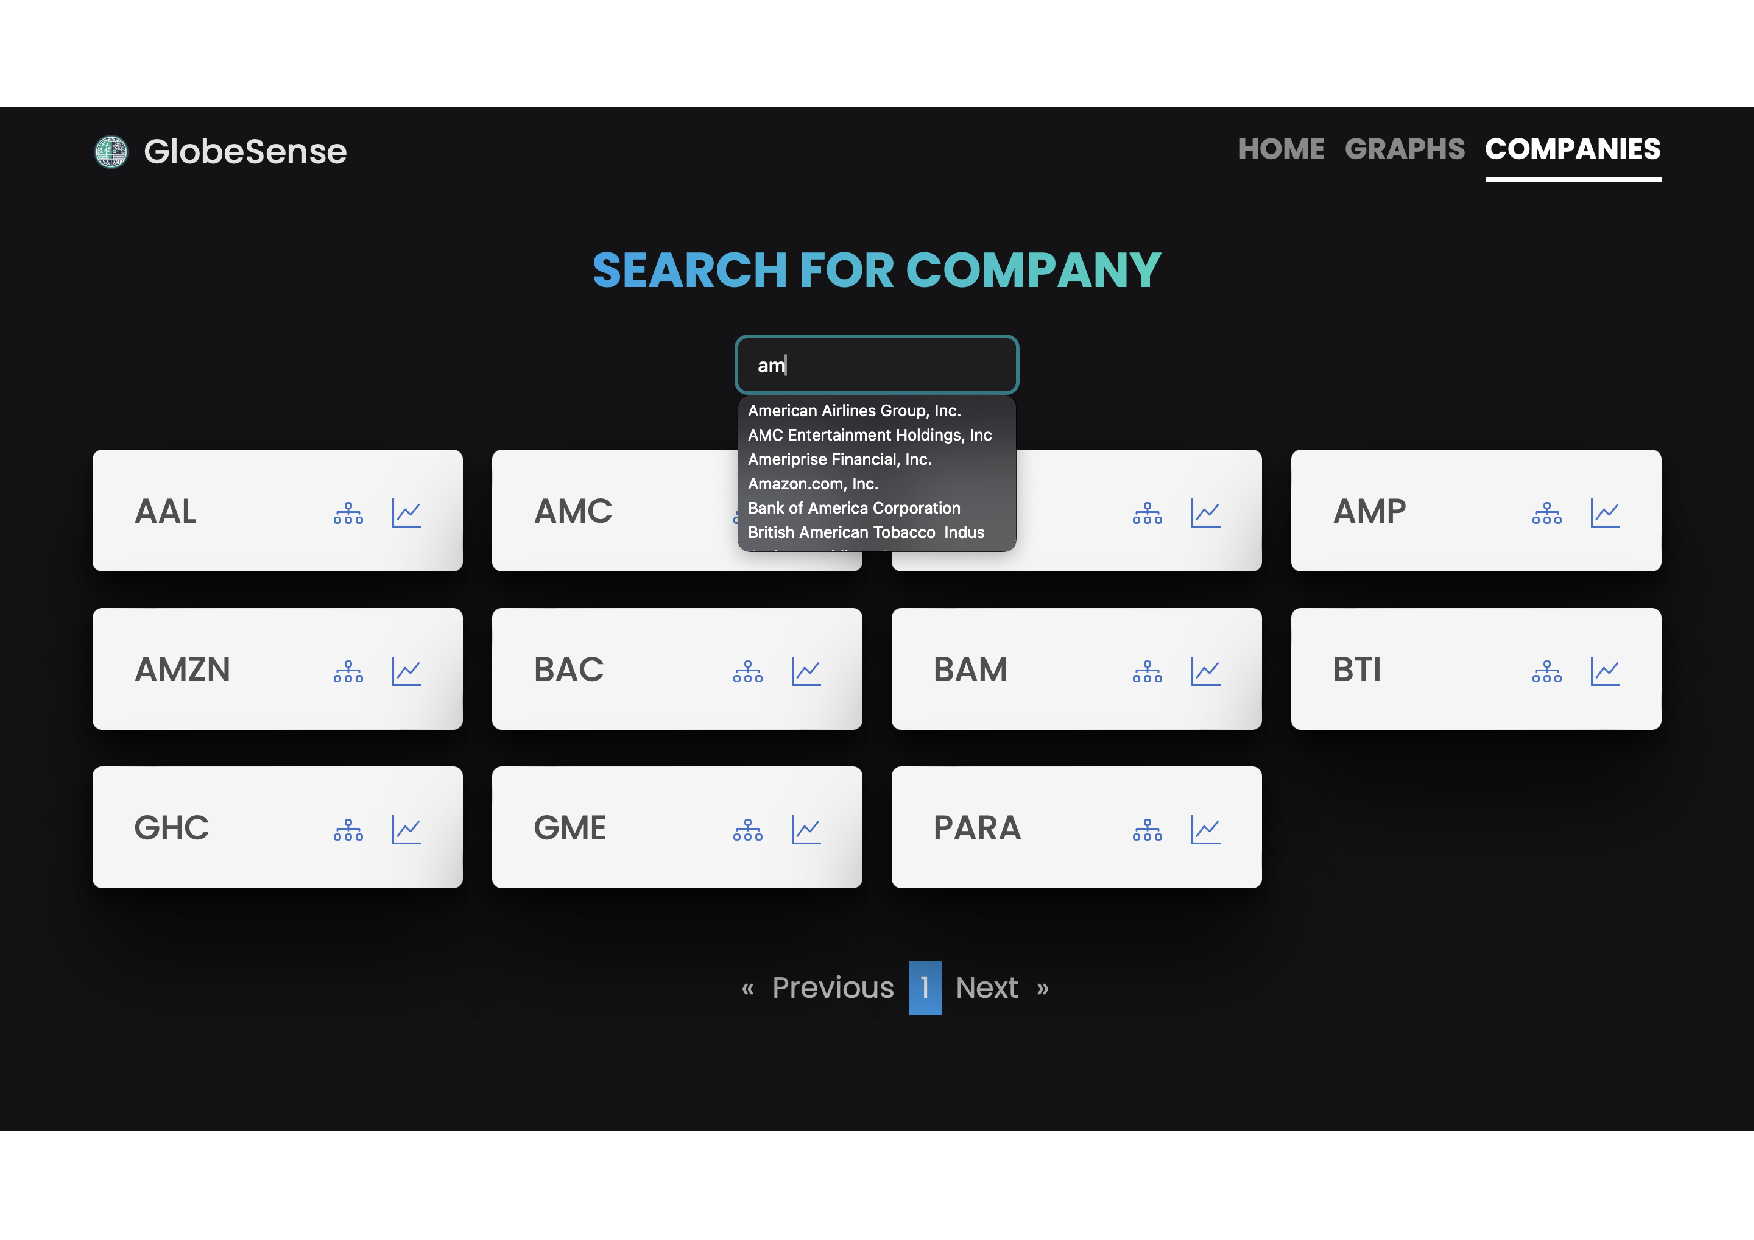
\includegraphics[width=\textwidth]{img/user/search-am-a.pdf}
    \caption{Companies search allows the users to search for a company by its name or stock symbol. The image shows the search for ``am''.}
    \label{fig:user-documentation-companies-search}
\end{figure}

\newpage

\section{Company Dashboard}
\label{sec:user-documentation-company-dashboard}
The company dashboard offers users comprehensive information about the company through multiple components (see Figure \ref{fig:comapny-apple}).

\begin{figure}[htbp]
    \centering
    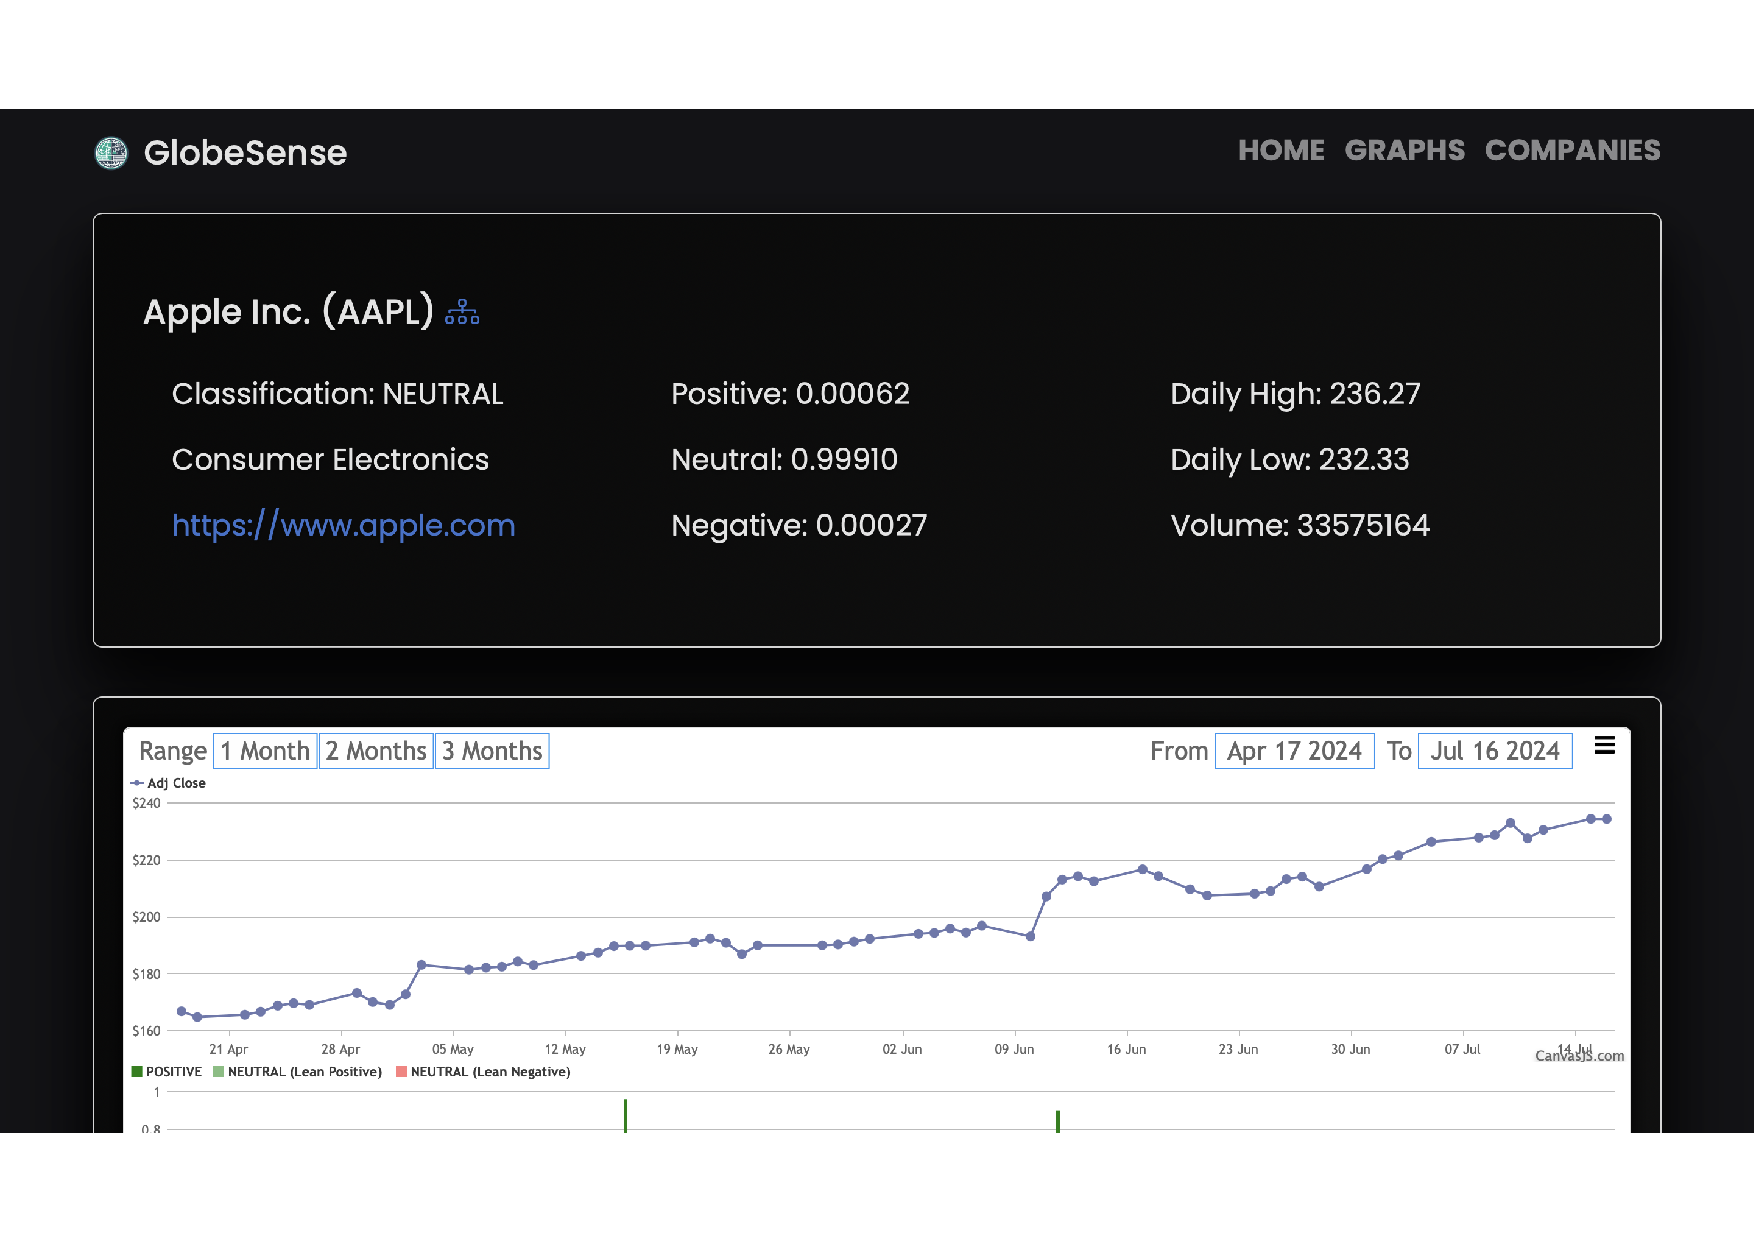
\includegraphics[width=\textwidth]{img/user/company-apple-a.pdf}
    \caption{Apple Inc. dashboard overview.}
    \label{fig:comapny-apple}
\end{figure}

\subsection{Company Information}
\label{subsec:company-information}
The company information component includes the company's name, stock symbol, and a graph link. It provides average daily sentiment values categorised as positive, neutral, or negative, updated every $4$ hours. Additionally, it displays Yahoo Finance data, including daily high, low, and volume, which is refreshed with each visit (see Figure \ref{fig:apple-info}).

\begin{figure}[htbp]
    \centering
    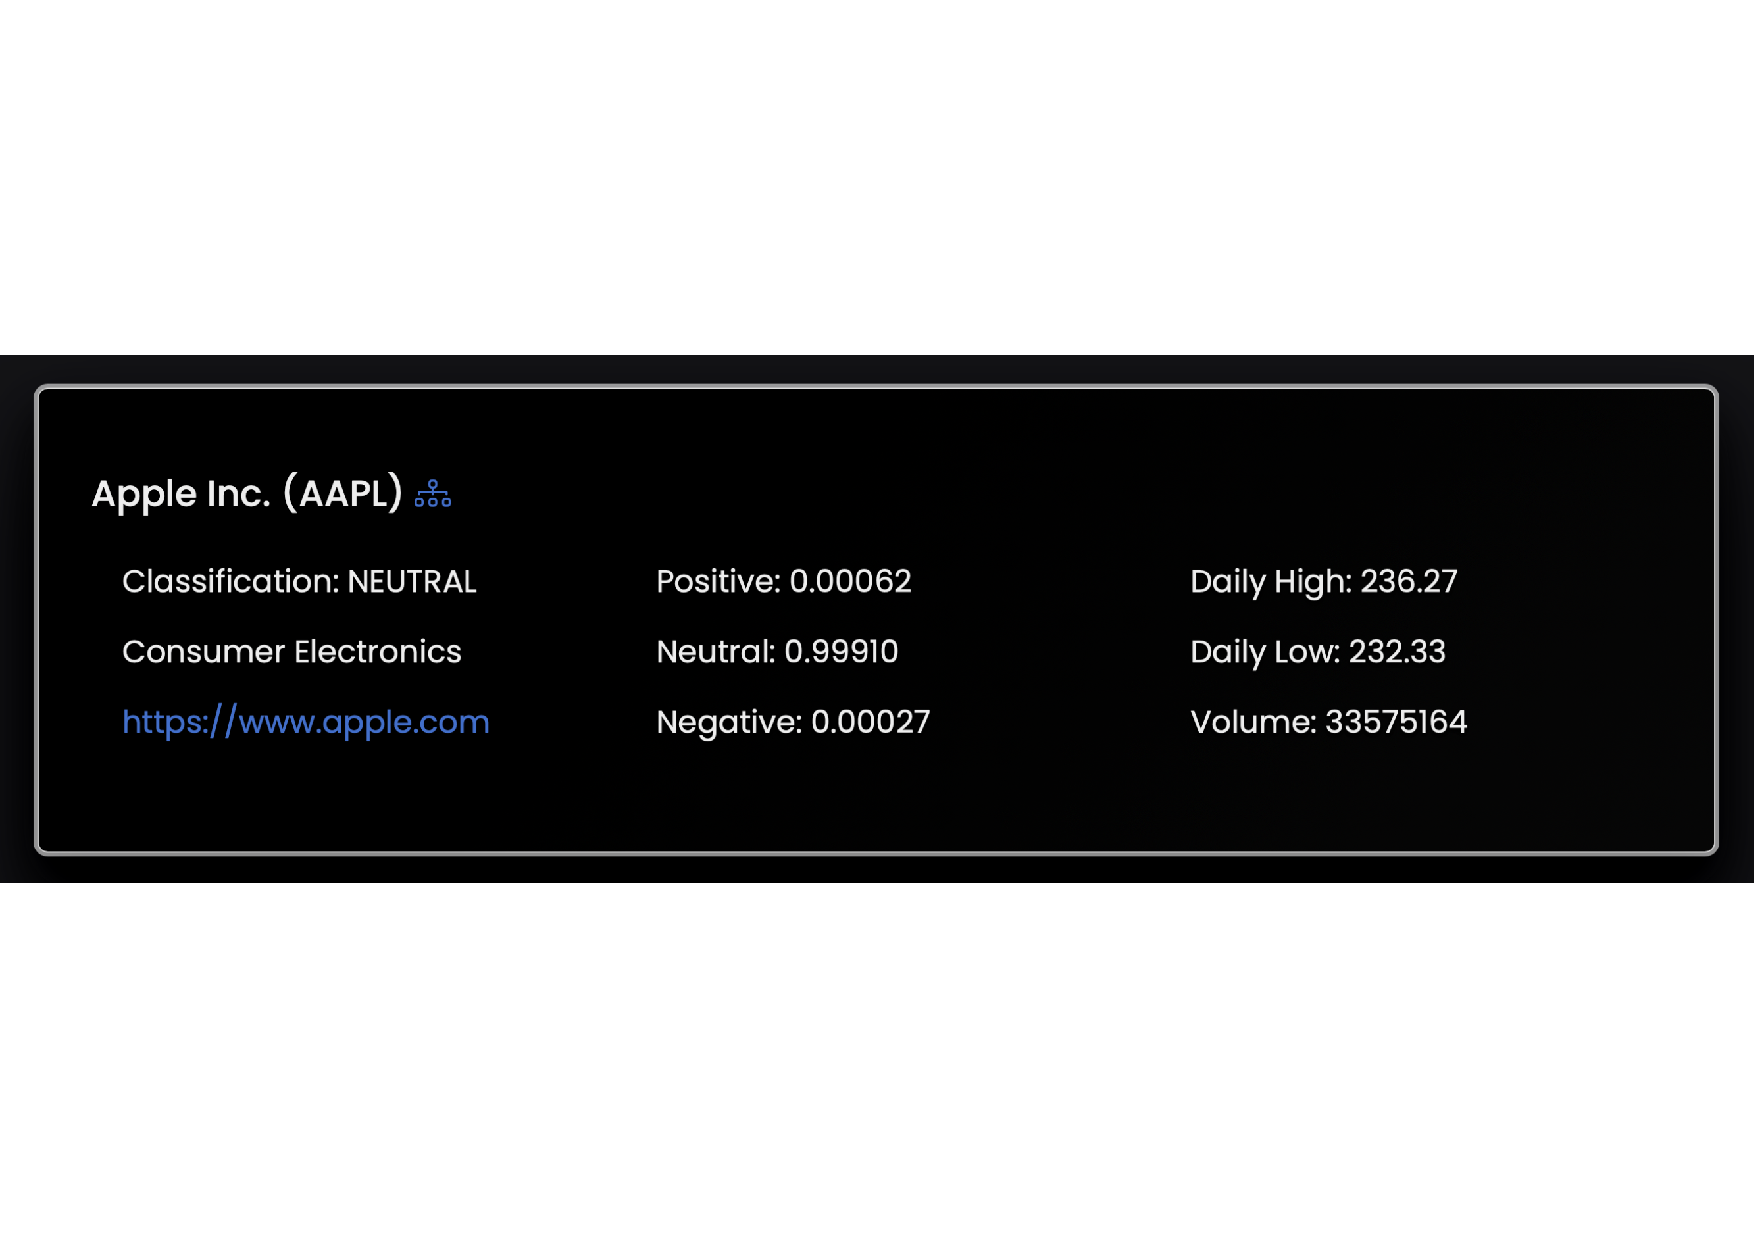
\includegraphics[width=\textwidth]{img/user/apple-info-a.pdf}
    \caption{Apple Inc. company information.}
    \label{fig:apple-info}
\end{figure}

\subsection{Stock Chart}
\label{subsec:stock-chart}
The stock chart component shows the adjusted close price of the company for the past three months. The users can zoom in and out by selecting the time range (see Figure \ref{fig:apple-stock}). The chart is divided into two parts; the upper part shows the price, and the lower part shows the daily average value of the company's sentiments in the articles for a given day.

Sentiments in the second part can be hidden by clicking on the sentiment legend. Hovering over the chart shows the date, stock price, and sentiment value for a given day (see Figure \ref{fig:apple-stock-range-neutral}).

\begin{figure}[htbp]
    \centering
    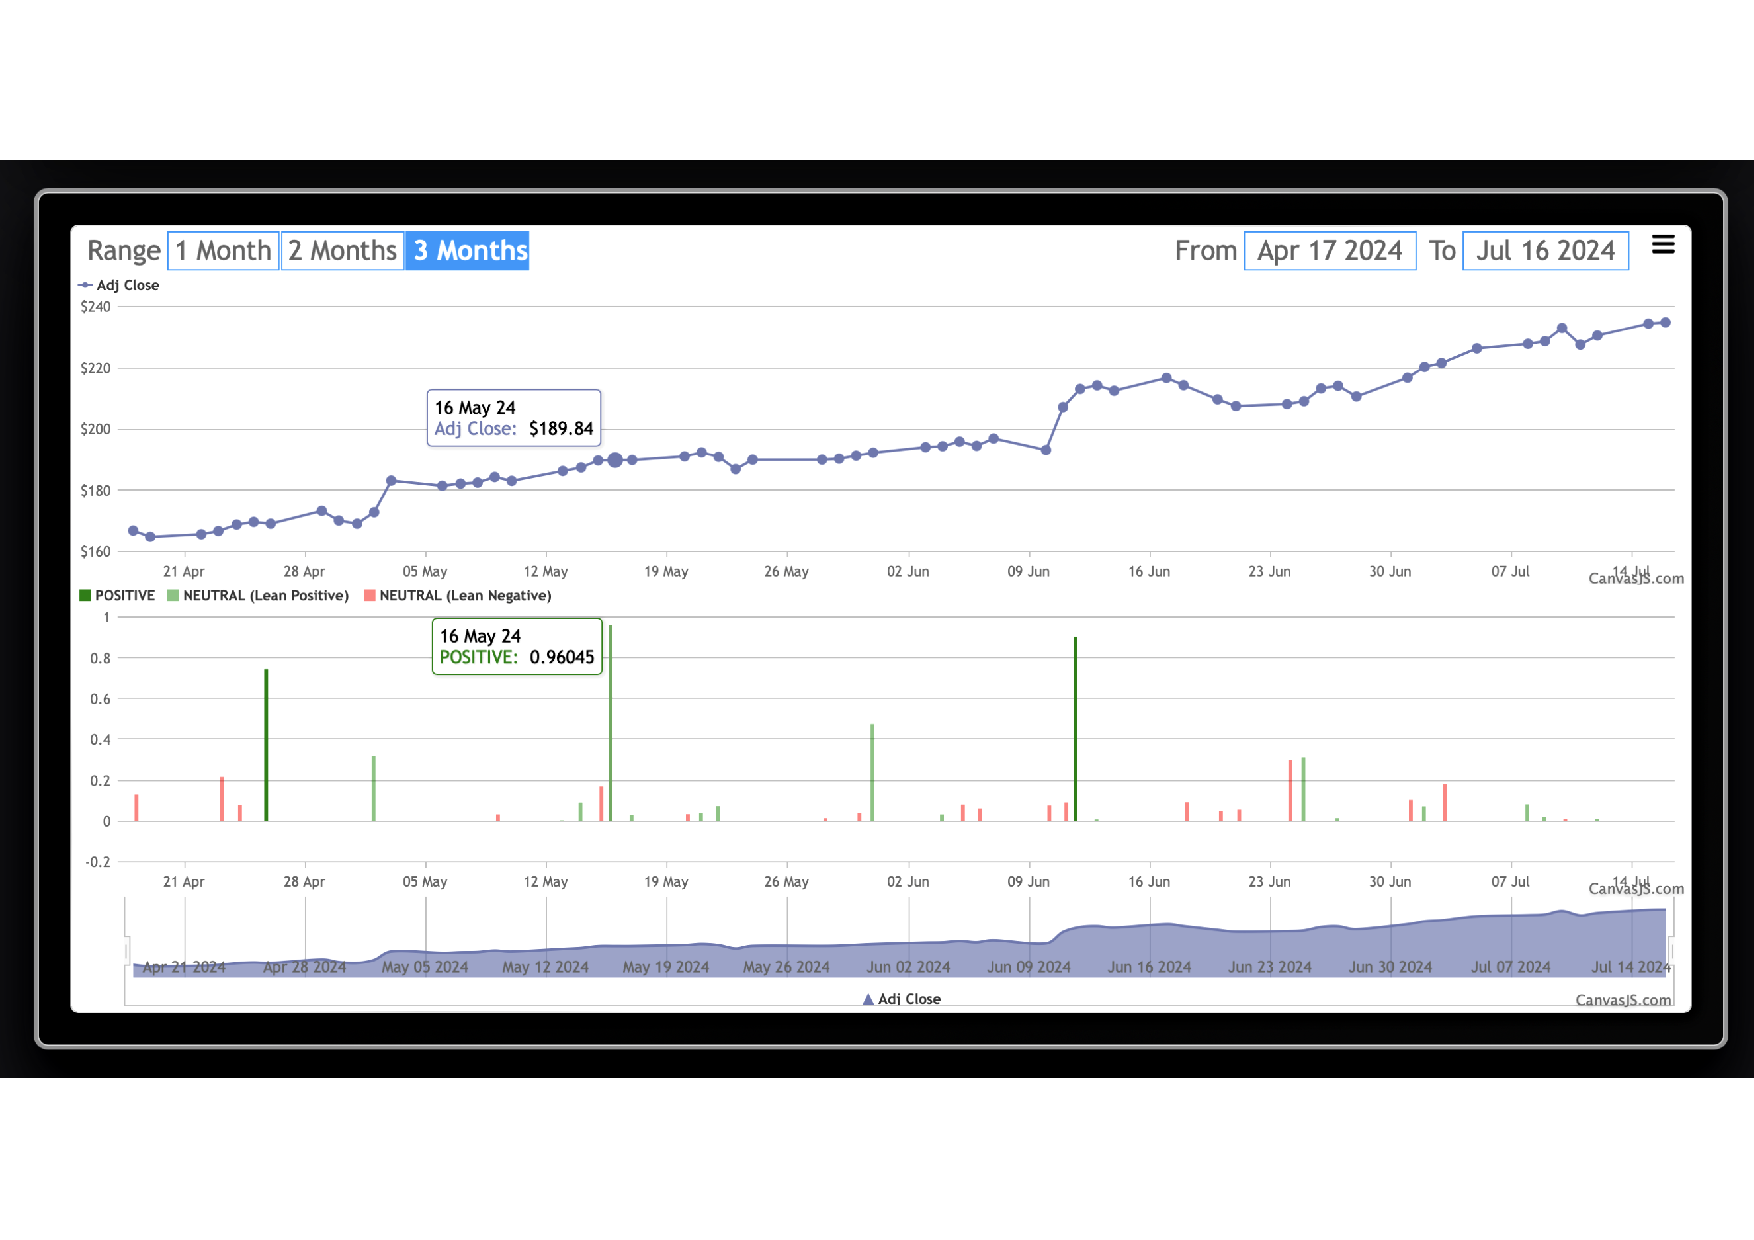
\includegraphics[width=\textwidth]{img/user/apple-stock-a.pdf}
    \caption{Apple Inc. stock chart in default view.}
    \label{fig:apple-stock}
\end{figure}

\begin{figure}[htbp]
    \centering
    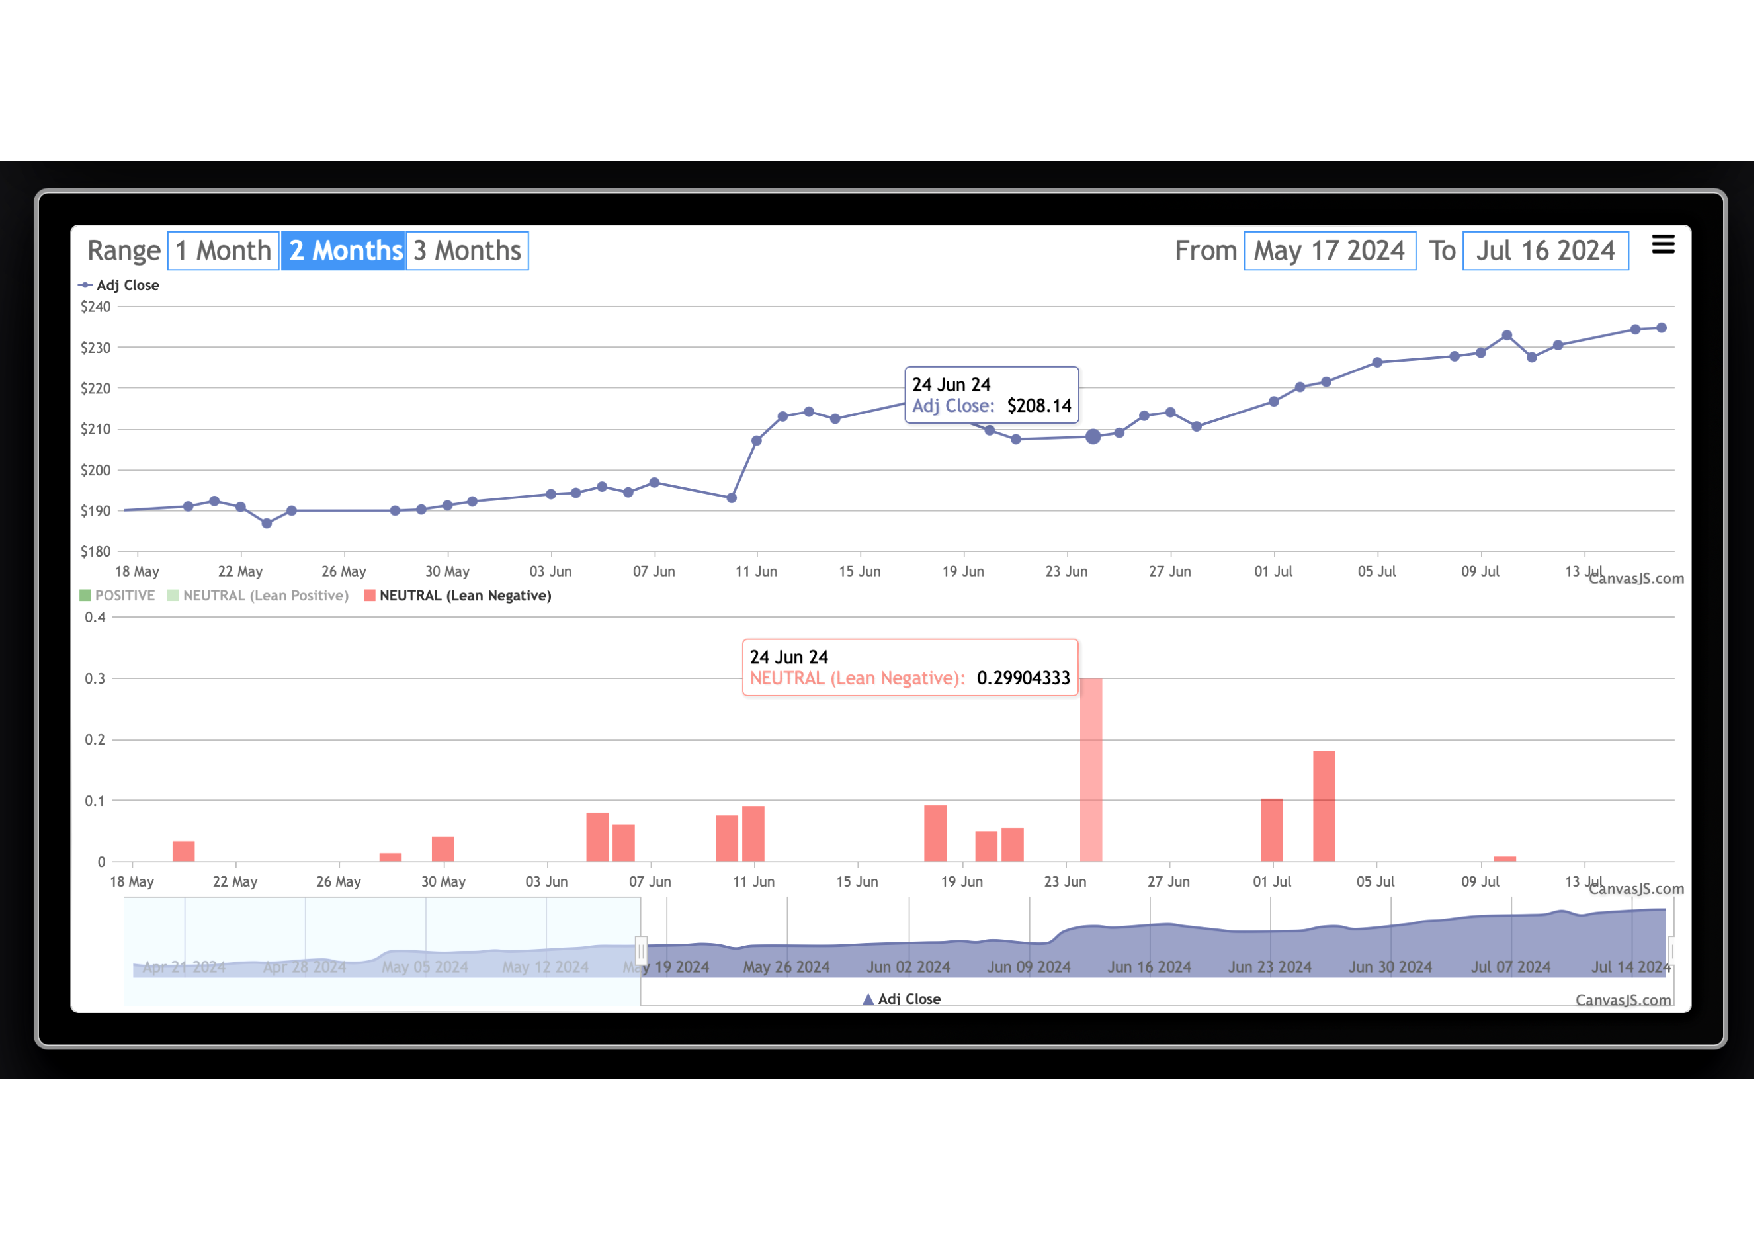
\includegraphics[width=\textwidth]{img/user/apple-stock-range-neutral-a.pdf}
    \caption{Apple Inc. stock chart in two months range with hidden sentiment values except neutral (lean negative).}
    \label{fig:apple-stock-range-neutral}
\end{figure}


\subsection{Spline Chart}
\label{subsec:spline-chart}
The spline chart component demonstrates the evolution of the daily average sentiment value over the past three months. Users can hide the sentiment spline like in the stock chart by clicking on the sentiment legend. Hovering over the chart shows a given day's date and sentiment value (see Figure \ref{fig:apple-stock-spline}).

\begin{figure}[htbp]
    \centering
    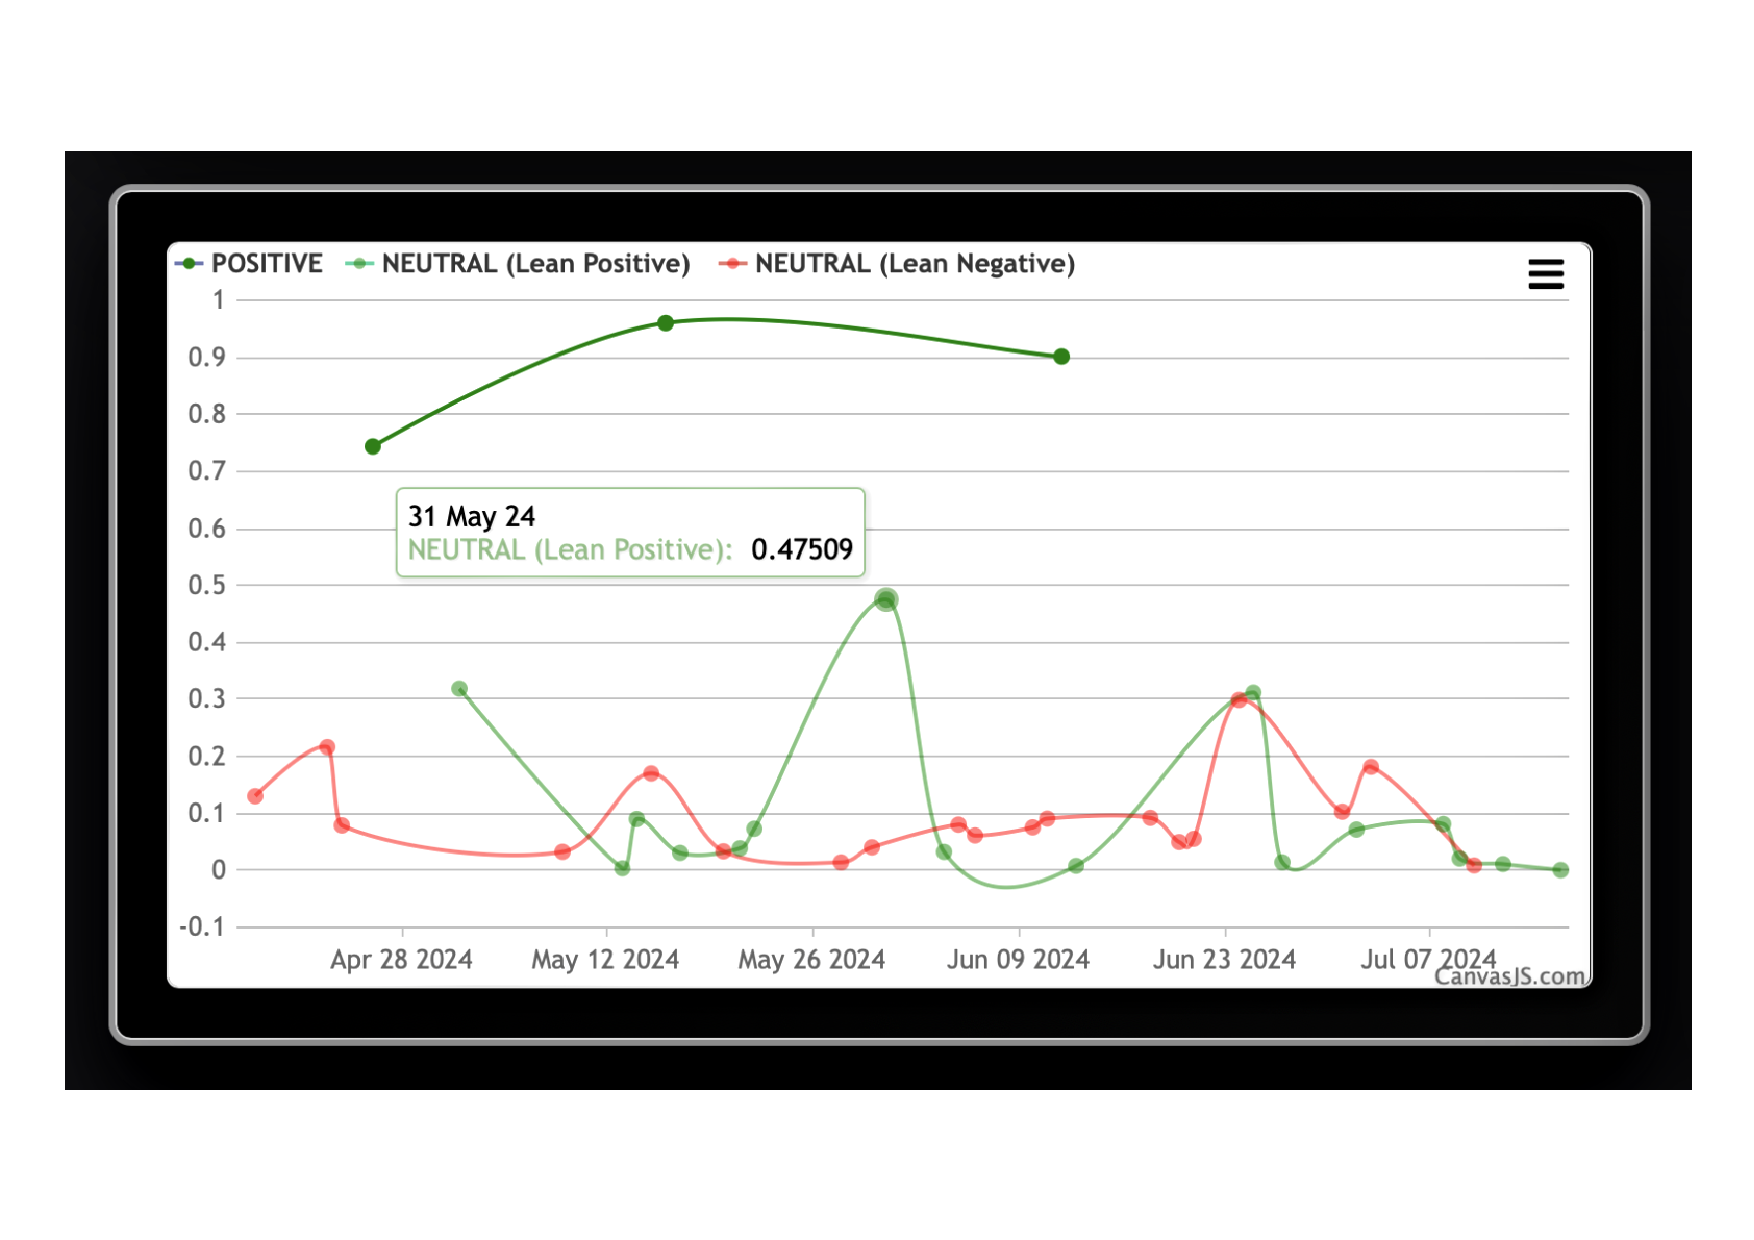
\includegraphics[width=\textwidth]{img/user/apple-spline-chart-a.pdf}
    \caption{Apple Inc. spline chart displaying the daily average sentiment value evolution for the past three months.}
    \label{fig:apple-stock-spline}
\end{figure}

\subsection{Pie Chart}
\label{subsec:pie-chart}
The pie chart component illustrates the daily average sentiment values distribution for the past three months (see Figure \ref{fig:apple-pie}).

\begin{figure}[htbp]
    \centering
    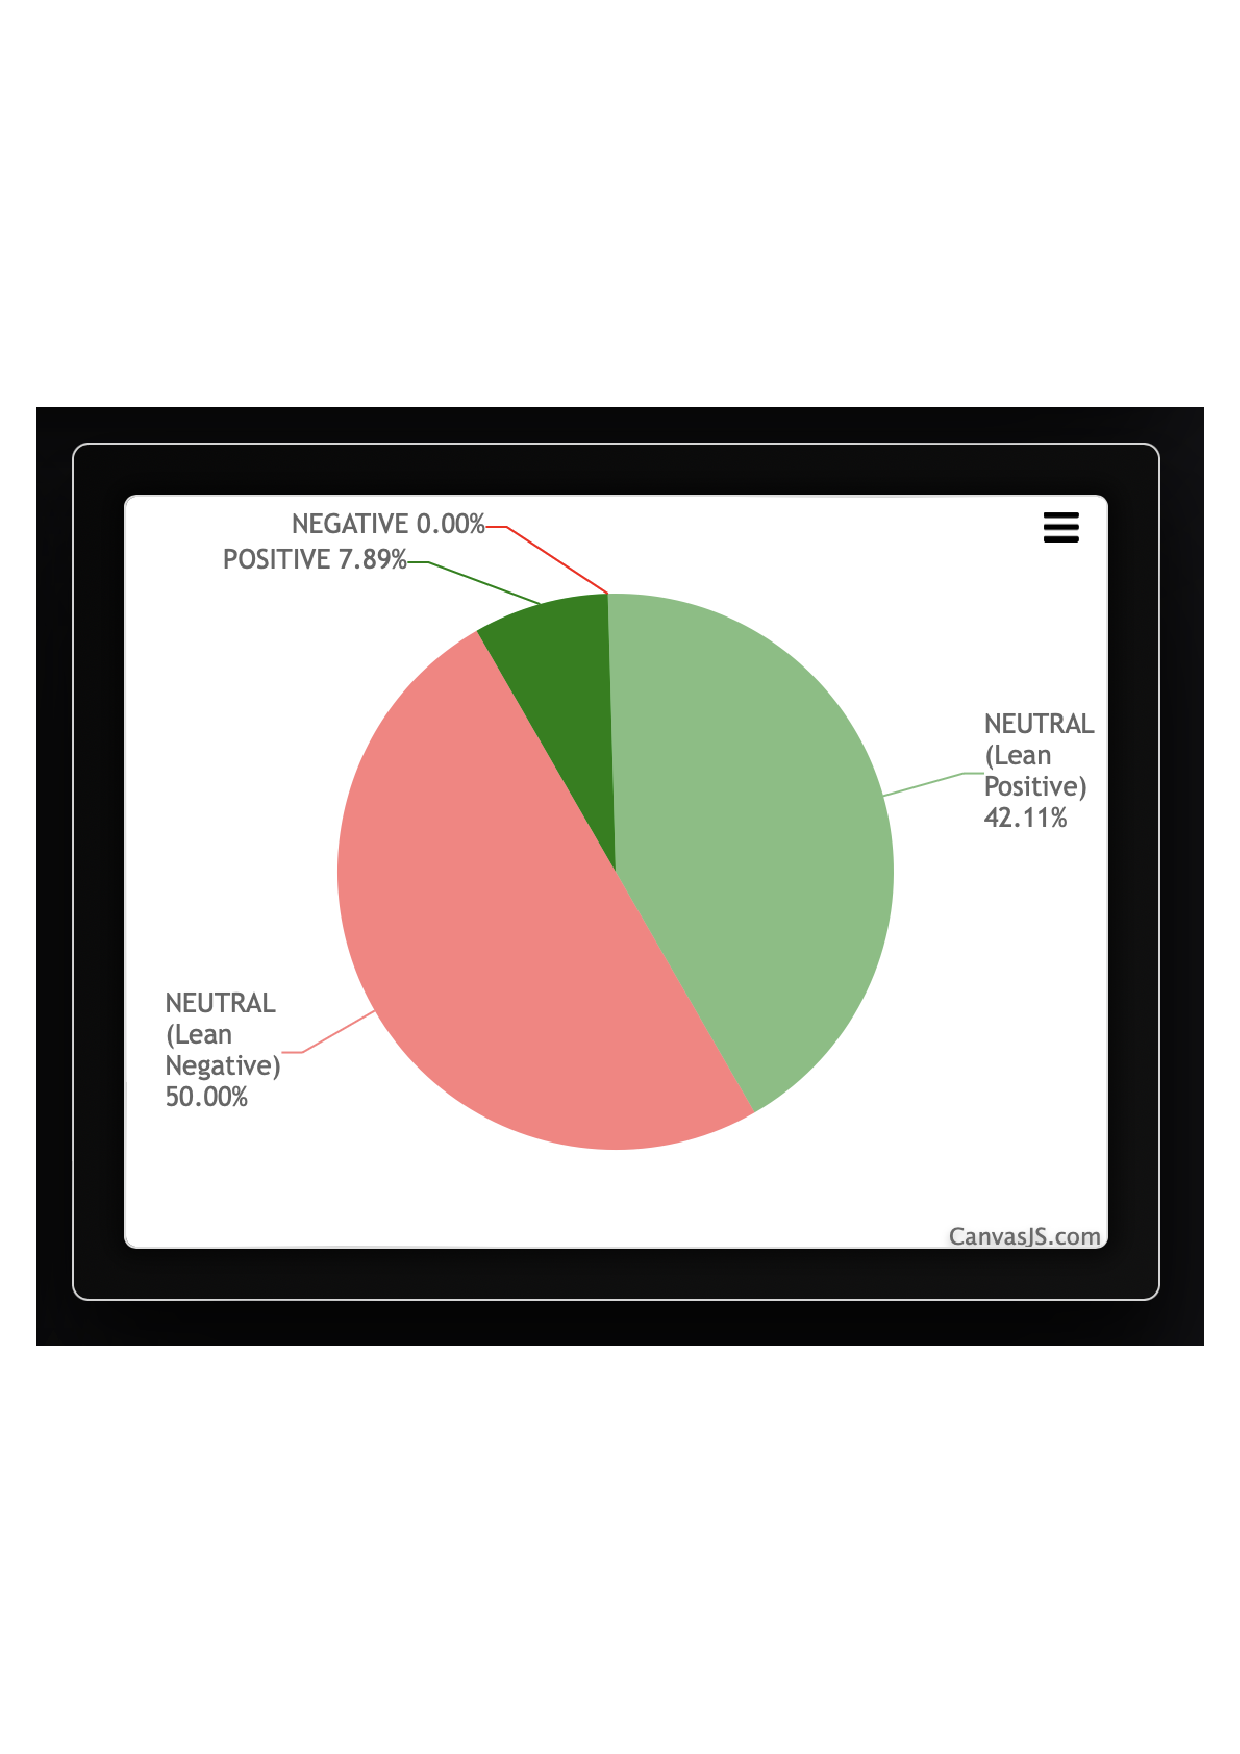
\includegraphics[width=0.8\textwidth]{img/user/apple-pie-chart-a.pdf}
    \caption{Apple Inc. pie chart showing the daily average sentiment values distribution for the past three months.}
    \label{fig:apple-pie}
\end{figure}

\subsection{Article List}
\label{subsec:article-list}
The article list component shows the list of articles in which the company is mentioned, along with the sentiment of the company in the article. Users can navigate to the article page by clicking on the article source website. 

It also provides the company's sentiment value in the article, which is the company's sentiment in that article. It is a classic pagination where users can navigate to the next or previous page. Overall, column ordering is allowed by clicking on the column name. Users can also filter the articles by the search terms in the search bar. Thus, the articles can be searched by title, author, type, specific sentiment classification, and more. See Figures \ref{fig:apple-articles-positive}, \ref{fig:apple-articles-date}, and \ref{fig:apple-articles-search}.

\begin{figure}[htbp]
    \centering
    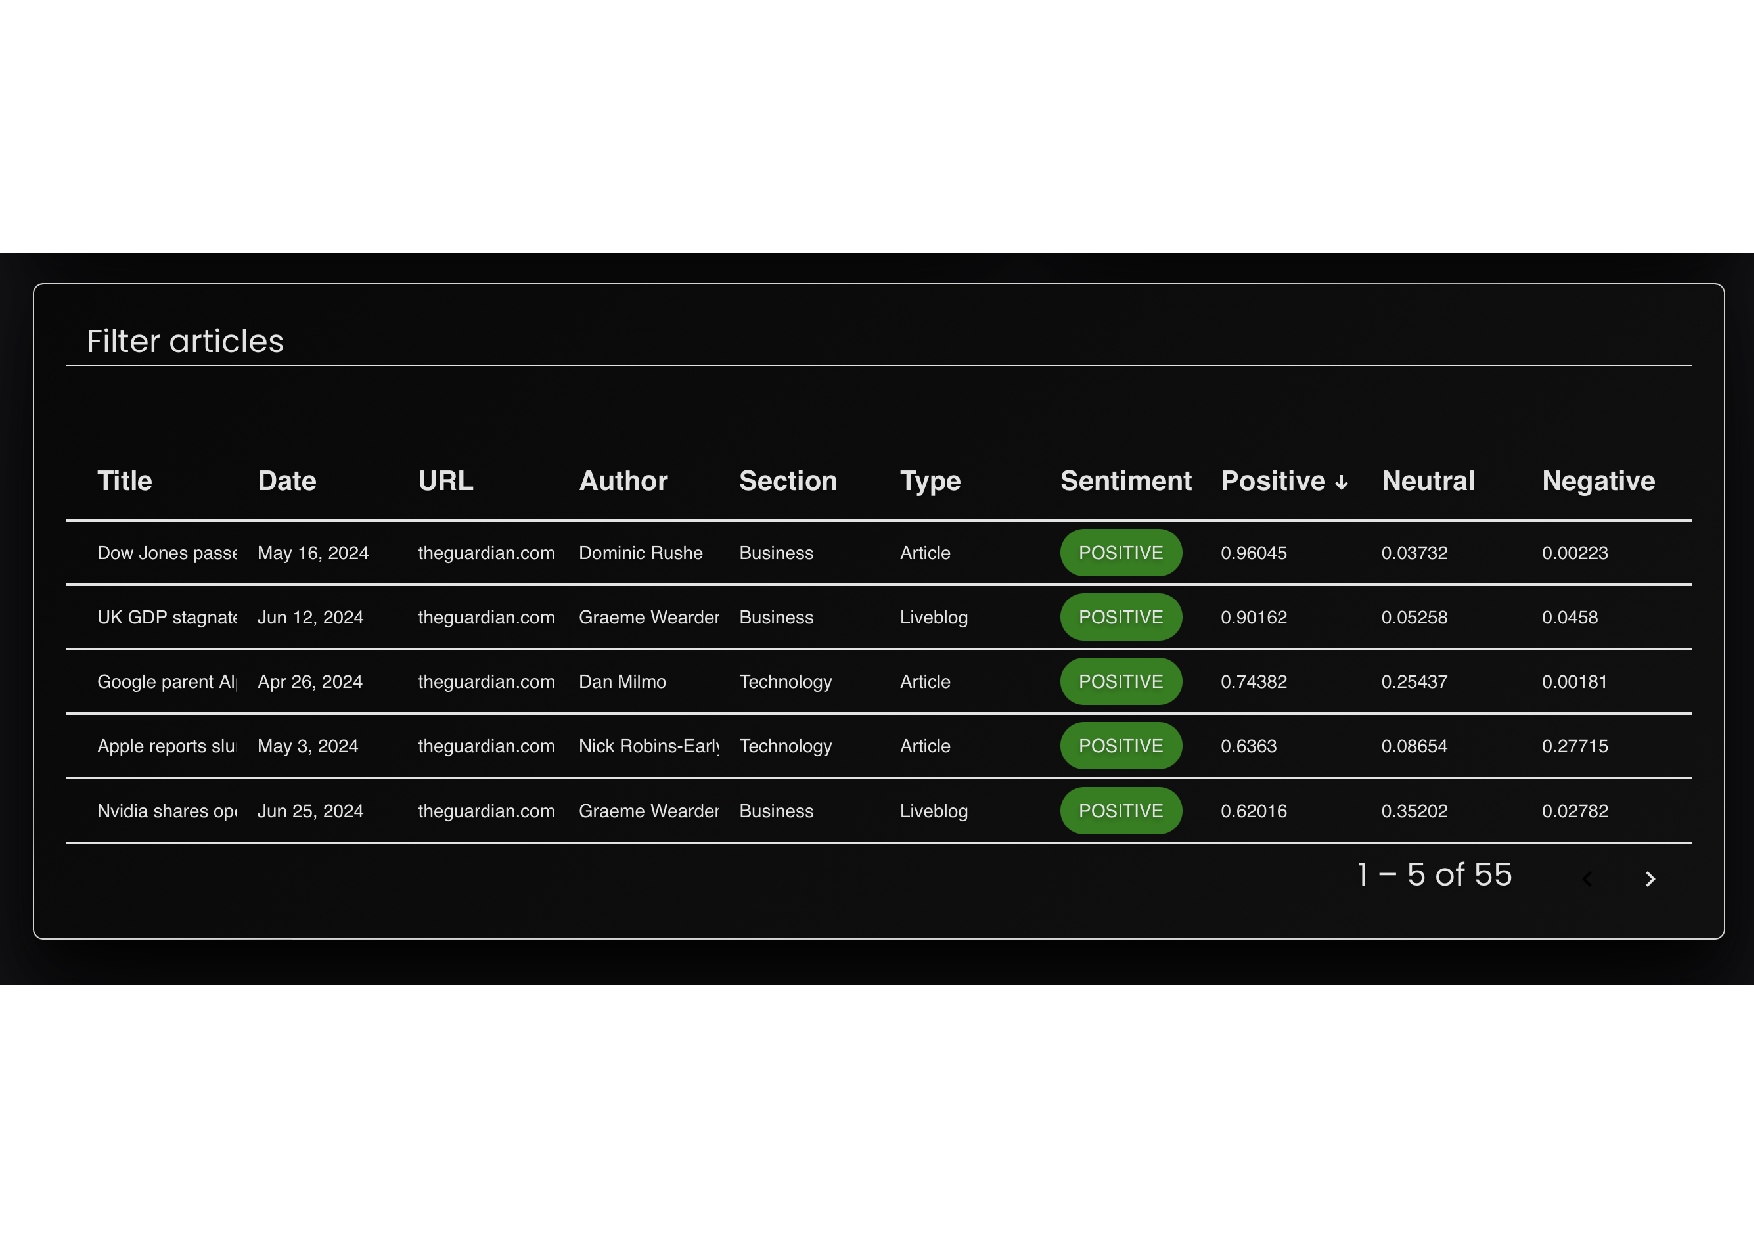
\includegraphics[width=\textwidth]{img/user/apple-articles-order-positive-a.pdf}
    \caption{Apple Inc. article list displaying the list of articles in which the company is mentioned with the sentiment of the company in the article in descending order by the positive sentiment value.}
    \label{fig:apple-articles-positive}
\end{figure}

\begin{figure}[htbp]
    \centering
    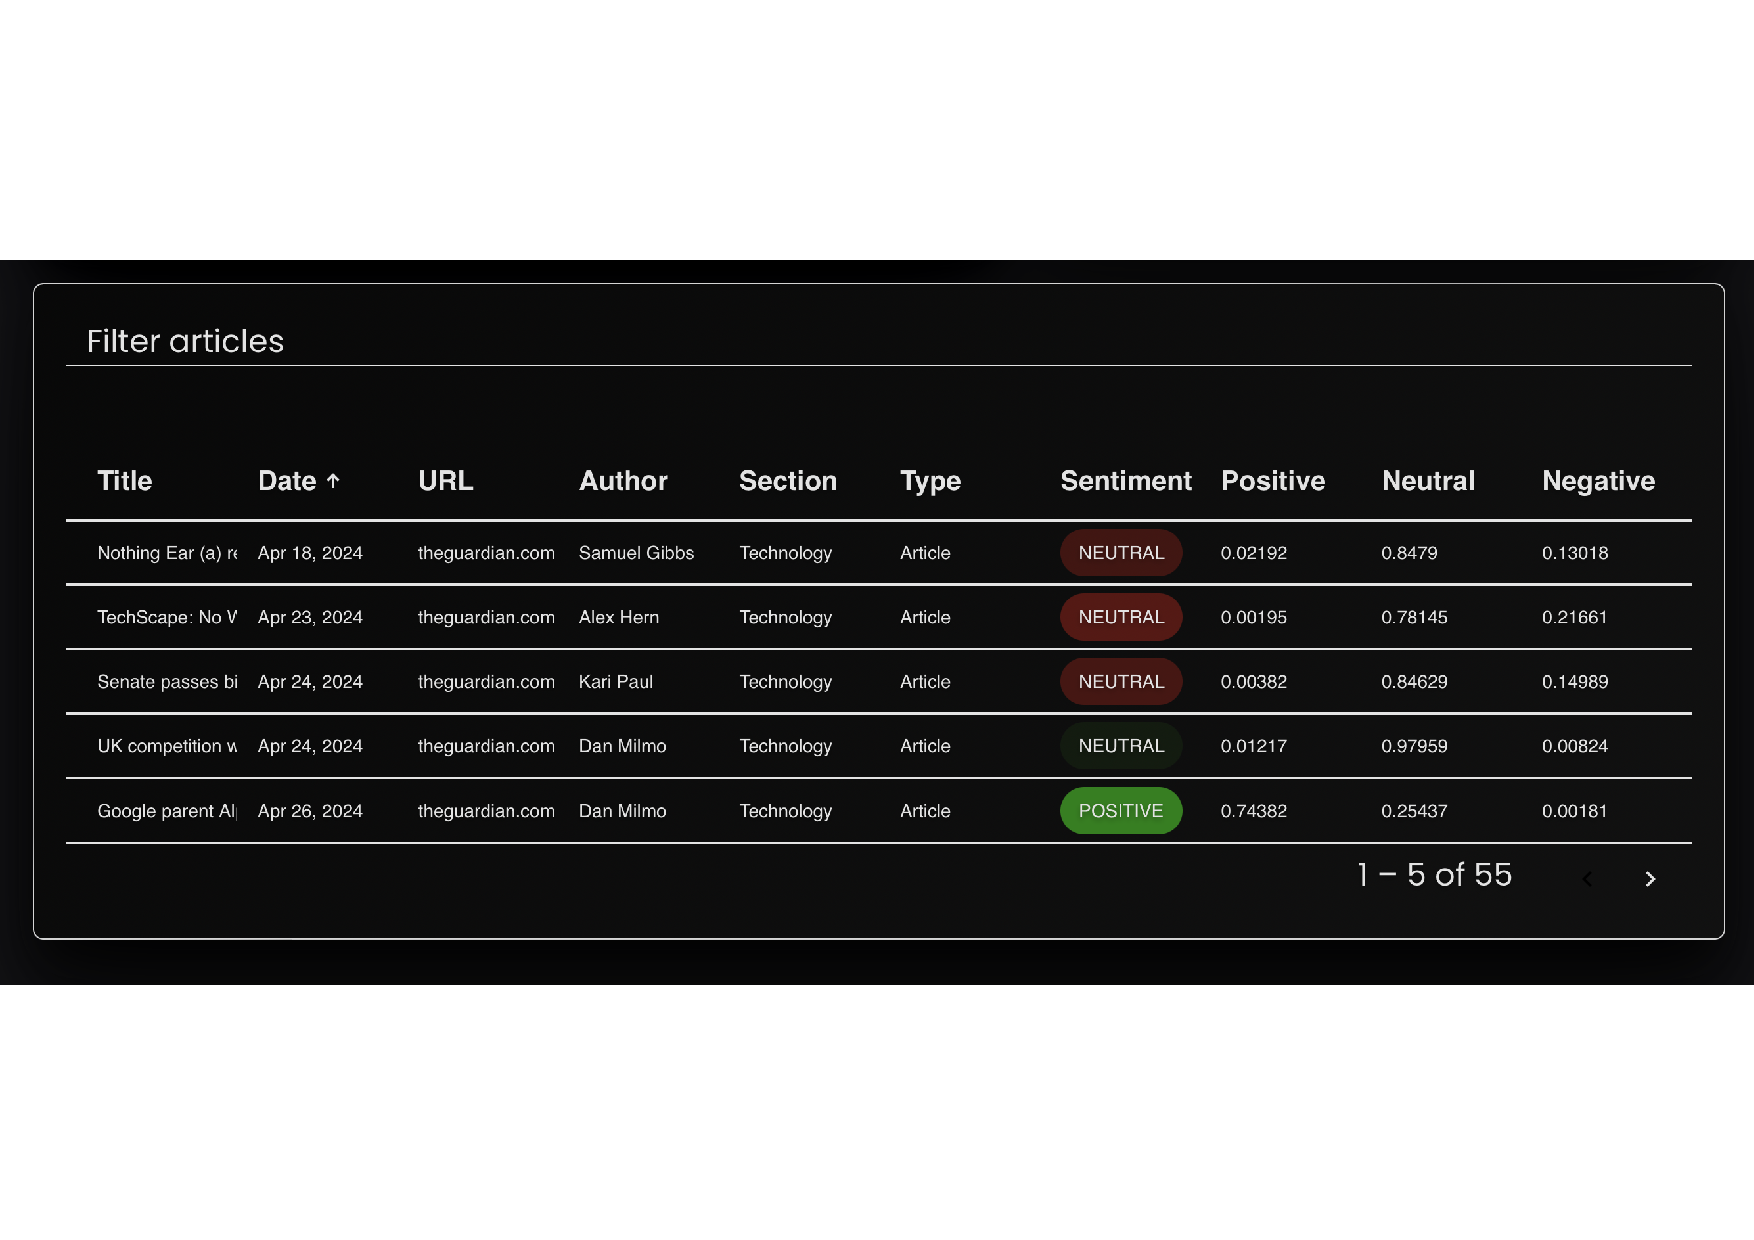
\includegraphics[width=\textwidth]{img/user/apple-articles-order-date-a.pdf}
    \caption{Apple Inc. article list depicting the list of articles in which the company is mentioned with the sentiment of the company in the article in the ascending order by the date.}
    \label{fig:apple-articles-date}
\end{figure}

\begin{figure}[htbp]
    \centering
    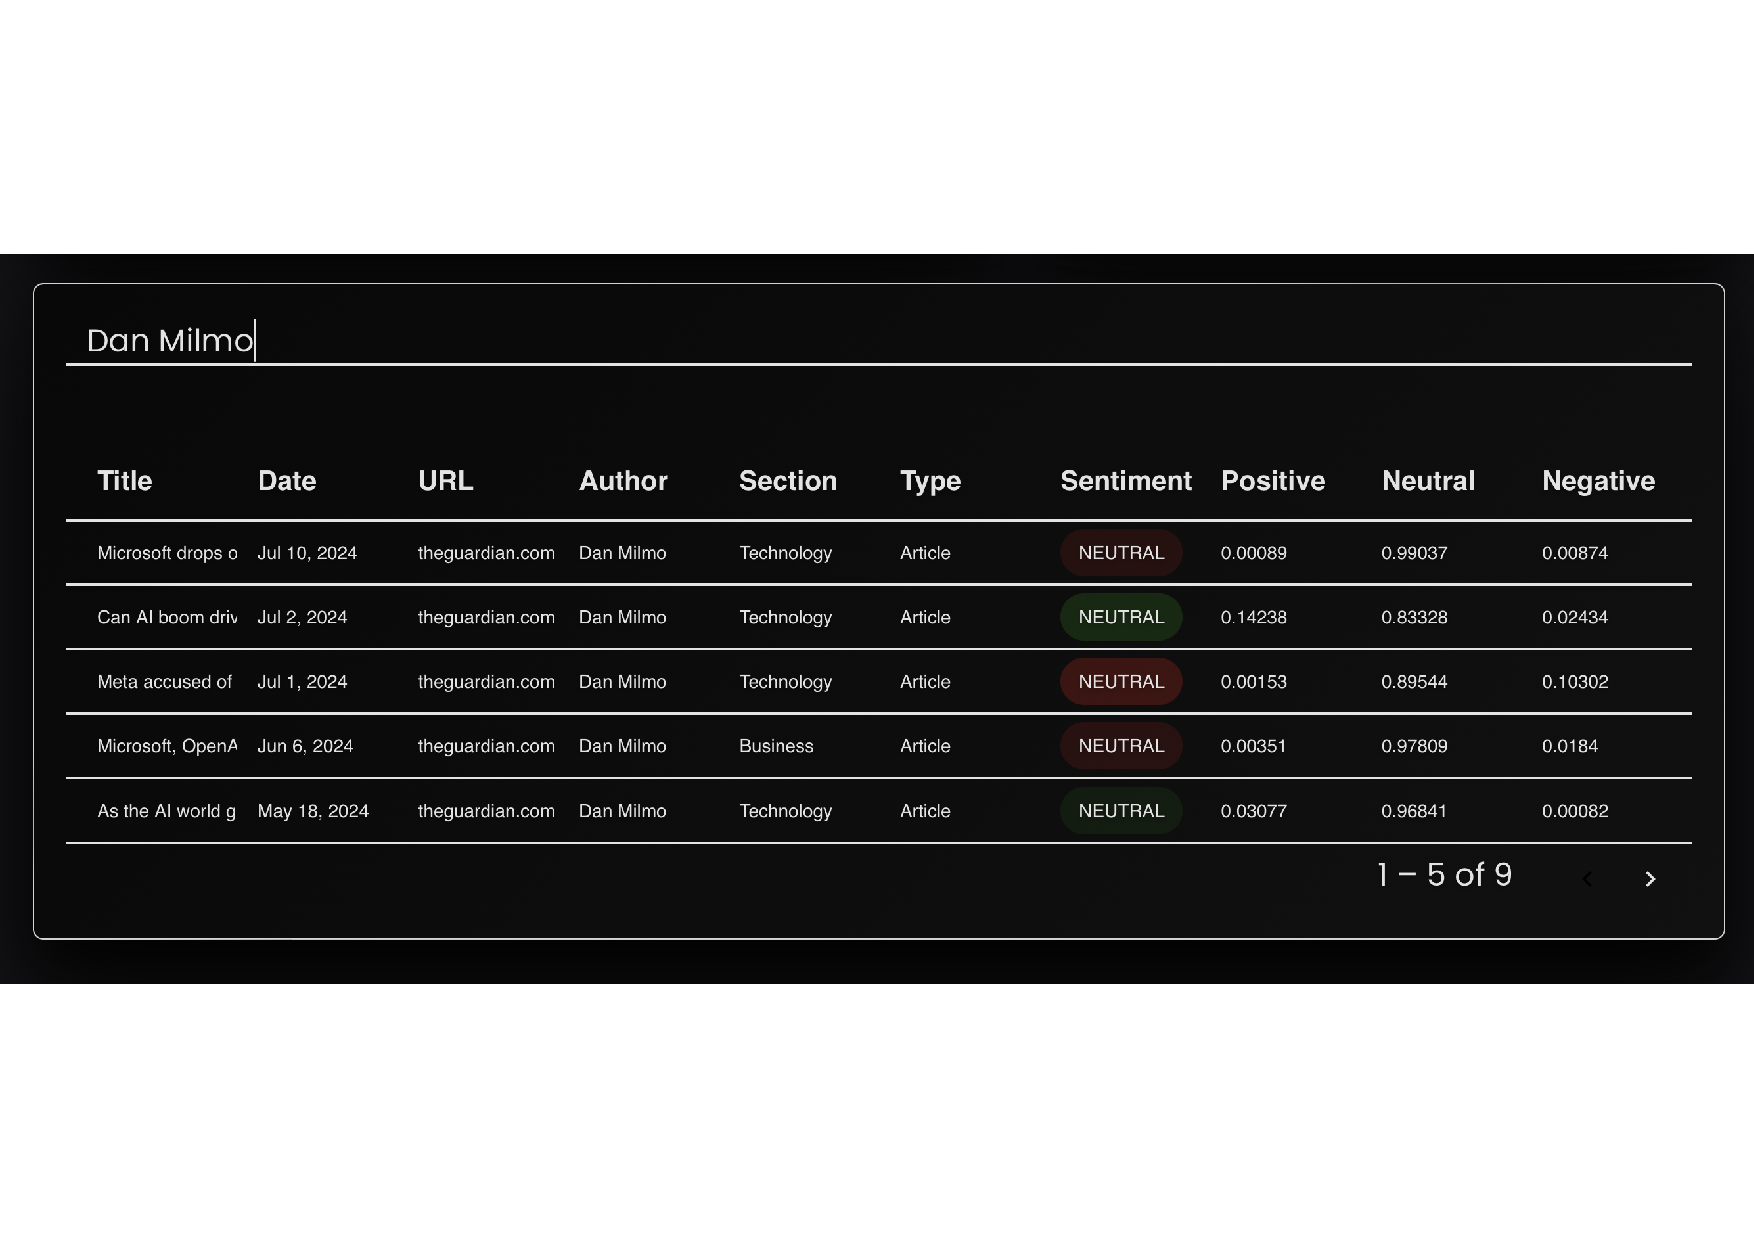
\includegraphics[width=\textwidth]{img/user/apple-articles-search-a.pdf}
    \caption{Apple Inc. article list portraying the list of articles in which the company is mentioned with the sentiment of the company in the article filtered by the search term ``Dan Milmo'' to find all articles written by the author.}
    \label{fig:apple-articles-search}
\end{figure}

\section{Company Graph}
\label{sec:user-documentation-company-graph}
The company graph page shows the network of all articles in which the company has been mentioned for the past three months. The edge shows by its colour the sentiment of the company within the article, which node is coloured by the sentiment associated with the company, unlike companies graphs where the average sentiment of all associated companies colours articles. Actions are the same as on the general graph page.

Hovering over a node displays its name in the case of a company and its title in the case of an article. In this case, it highlights only the article and company node, including the edge, after hovering over the article. Hovering the company node just increases (highlights) its size but not relationships with all articles, which is unnecessary in this projection type. The user can navigate the article page by clicking the article node (see Figure \ref{fig:user-documentation-company-graph}).

The general control panel has a purpose similar to that of the graphs page. Visibility and distances remain the same. The company and article node control panel provides the following details:

\begin{itemize}
    \item \textbf{Article node}
    \begin{itemize}
        \item \textbf{Title} - the title of the article.
        \item \textbf{Published date} - the date when the article was published.
        \item \textbf{Author} - the author of the article.
        \item \textbf{Open article} - the link to the article.
        \item \textbf{Sentiment} - the sentiment of the company in the article.
    \end{itemize}
    \item \textbf{Company node}
    \begin{itemize}
        \item \textbf{Company information} - the details about the company, such as a ticker and link to the company's dashboard. Additionally, it presents the average daily sentiment of the company.
        \item \textbf{Articles} - the list of articles in which the company is mentioned with the sentiment of the company in the article.
    \end{itemize}
\end{itemize}

\begin{figure}[hb]
    \centering
    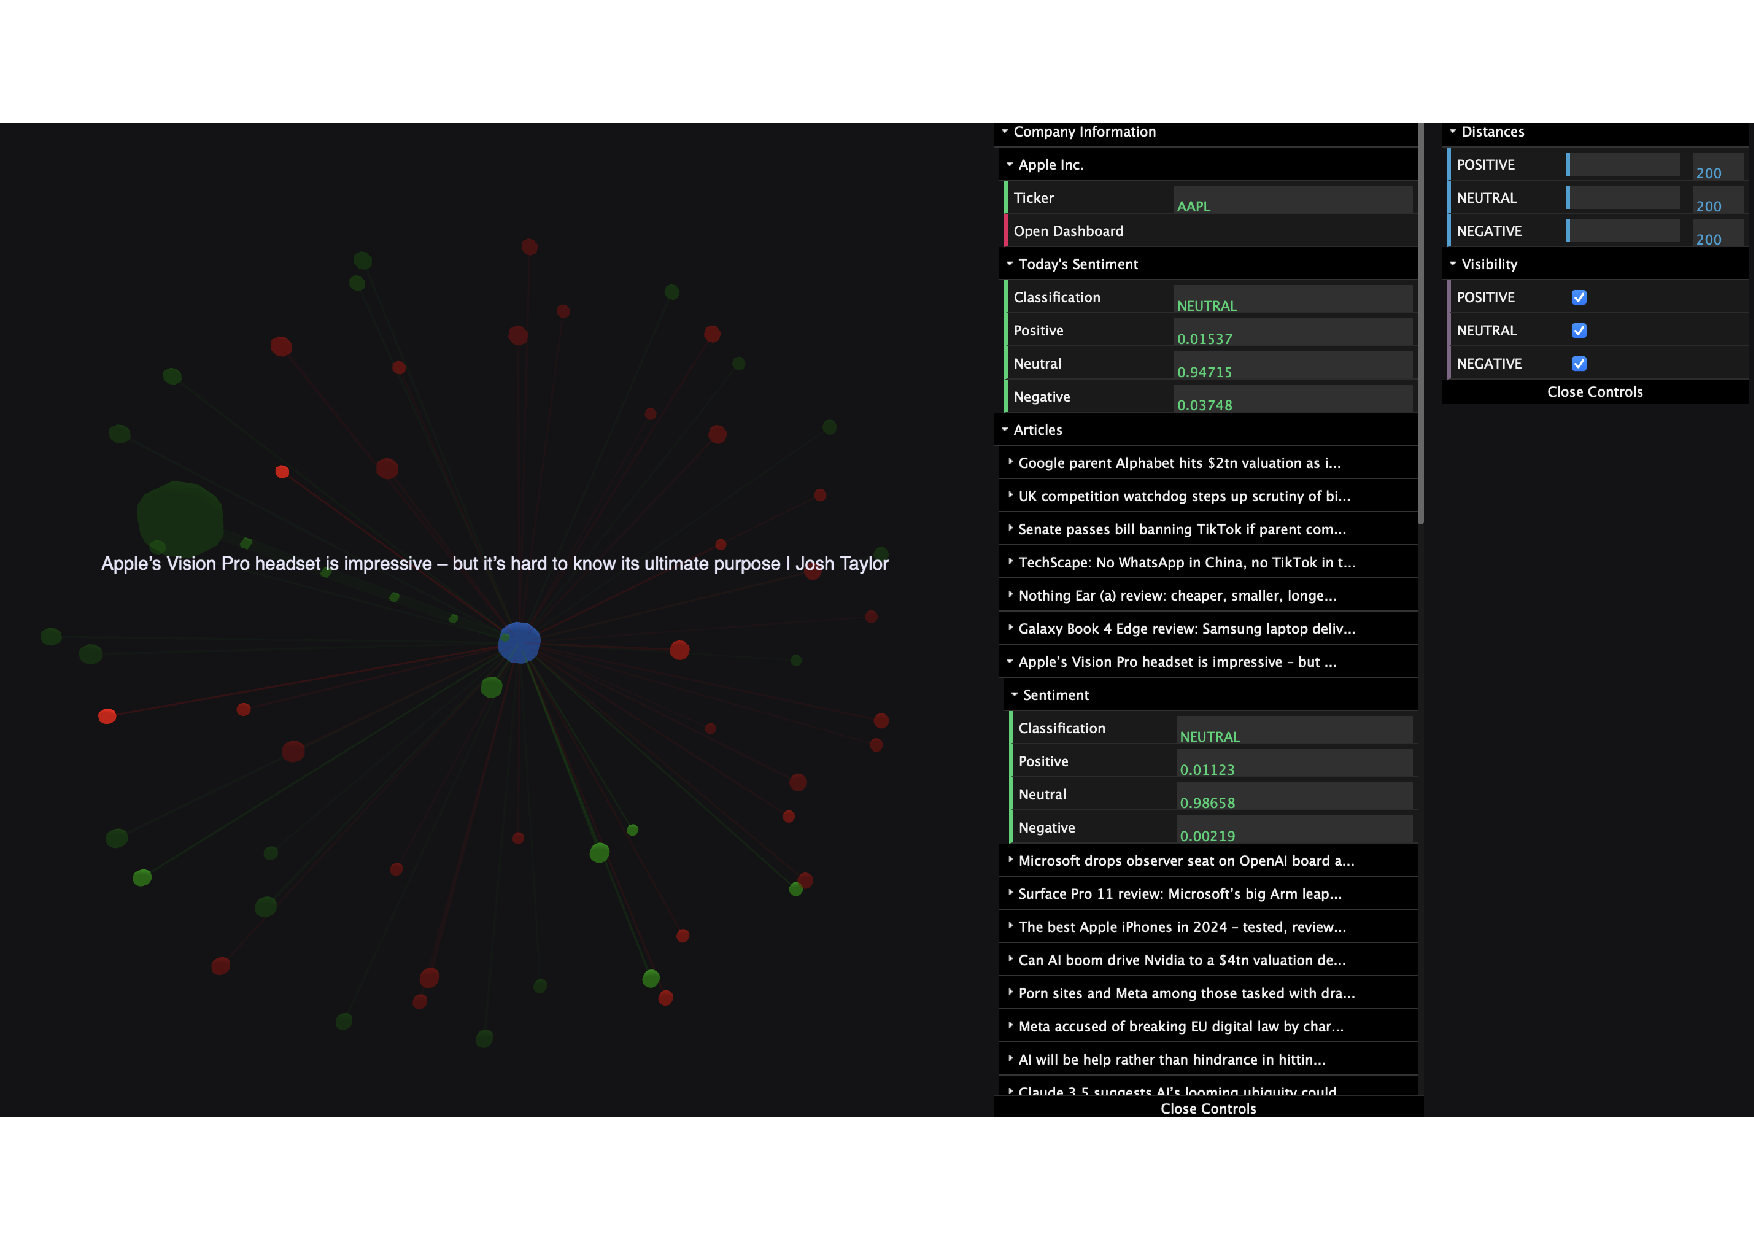
\includegraphics[width=\textwidth]{img/user/apple-company-graph-a.pdf}
    \caption{Apple Inc. company graph displaying the network of all articles mentioned in the company for the past three months. The state after clicking on the company node and hovering over article node is illustrated.}
    \label{fig:user-documentation-company-graph}
\end{figure}
 